\documentclass[fontsize=11pt,chapterprefix=false,headings=big,headsepline=on,paper=5.500in:8.50in,DIV=11,BCOR=5mm,parskip=half+]{scrbook}
\usepackage{soul}
\usepackage[utf8]{inputenc}
\usepackage[T1]{fontenc}
\usepackage[spanish,mexico]{babel}
%\usepackage{lmodern}
%%%%%%% Conjunto DejaVu
%\usepackage{DejaVuSerifCondensed}
%\usepackage{DejaVuSansCondensed}
%\usepackage{DejaVuSansMono}
%%%%%%% Alegreya y Pandora
\usepackage{Alegreya}
\usepackage{AlegreyaSans}
\usepackage{inconsolata}
%%%%%%% Source Pro
% \usepackage{sourceserifpro}
% \usepackage{sourcesanspro}
% \usepackage{sourcecodepro}
\usepackage{textcomp}
\usepackage{hologo}
% \usepackage[outer=3in,inner=1.5in,top=1.5in,bottom=2.5in]{geometry}
\usepackage[spanish=mexican]{csquotes}
\usepackage{graphicx}
\graphicspath{{images/}}
\usepackage{url}
\def\UrlBreaks{\do\/\do\a\do\b\do\c\do\d\do\e\do\f\do\g\do\h\do\i\do\j\do\k\do\l\do\m\do\n\do\o\do\p\do\q\do\r\do\s\do\t\do\u\do\v\do\w\do\x\do\y\do\z\do\A\do\B\do\C\do\D\do\E\do\F\do\G\do\H\do\I\do\J\do\K\do\L\do\M\do\N\do\O\do\P\do\Q\do\R\do\S\do\T\do\U\do\V\do\W\do\X\do\Y\do\Z\do\%\do0\do1\do2\do3\do4\do5\do6\do7\do8\do9\do=\do/\do.\do:}
\usepackage{xcolor}
\usepackage{booktabs}
\usepackage{layout}
\usepackage[draft]{typogrid}
\typogridsetup{columns=1}

\usepackage{hyperref}
\hypersetup{
    pdftoolbar=true,        % show Acrobat’s toolbar?
    pdfmenubar=true,        % show Acrobat’s menu?
    pdffitwindow=false,     % window fit to page when opened
    pdfstartview={FitH},    % fits the width of the page to the window
    pdftitle={Lee esto 	para hacer un cambio real},    % title
    pdfauthor={Ángel Moma},     % author
    pdfsubject={Wikipolitica},   % subject of the document
    pdfcreator={Aradenatorix},   % creator of the document
    pdfproducer={Listopad}, % producer of the document
    pdfkeywords={} {} {} {}, % list of keywords
    pdfnewwindow=true,      % links in new window
    colorlinks=true,       % false: boxed links; true: colored links
    linkcolor=red,          % color of internal links (change box color with linkbordercolor)
    citecolor=green,        % color of links to bibliography
    filecolor=magenta,      % color of file links
    urlcolor=cyan           % color of external links
}

\usepackage[colorinlistoftodos,textsize=scriptsize,spanish]{todonotes}

\newcommand{\didit}[1]{\todo[color=red!40]{#1}} % Indica que esta parte ya está concluida
\newcommand{\revquotes}[1]{\todo[color=red!95]{Homologar criterio de uso de las comillas.}}
\newcommand{\addref}[1]{\todo[color=red!90]{[Cita requerida, #1]}} % Indica que hace falta una cita
\newcommand{\rewrite}[1]{\todo[color=green!40]{#1}} % Nota para comentar que hay que reescribir algo

\makeatletter
\if@todonotes@disabled
\newcommand{\hlfix}[2]{#1}
\else
\newcommand{\hlfix}[2]{\texthl{#1}\todo{#2}}
\fi
\makeatother% Resalta texto a corregir y agrega una nota alusiva al margen

\renewcommand*{\dictumwidth}{0.46\textwidth}

\setcounter{secnumdepth}{4}
\setcounter{tocdepth}{4}

\raggedbottom
\clubpenalty=10000 % Ajuste de tolerancia de líneas huerfanas
\widowpenalty=1000 % Ajuste de tolerancia de líneas viudas

\extratitle{Wikipolítica\\ \rule[0.5ex]{\textwidth}{0.5pt} \hfill Lee esto para hacer un cambio real}
\titlehead{Disonancias}
\subject{Wikipolítica}
\title{Lee esto}
\subtitle{para hacer un cambio real}
\author{Ángel Moma}
\date{\today}
\publishers{\emph{Listopad}}
\uppertitleback{\footnotesize
Primera edición, 2020. \\ 

\textcopyright{} \oldstylenums{2020} Ángel Moma\\
}

\lowertitleback{\footnotesize\raggedright
Diseño, edición y composición: \emph{Listopad} \\

La composición tipográfica se realizó con Pandoc y \hologo{LuaLaTeX}, mediante el uso de la colección \hologo{KOMAScript} sobre \hologo{LaTeXe}.\\

Los tipos usados en la presente edición son Alegreya y \textsf{Alegreya Sans}, diseñados por Juan Pablo del Peral, para \href{https://www.huertatipografica.com/es}{Huerta Tipográfica}, que se encuentran disponibles en \url{https://github.com/huertatipografica/Alegreya} y \url{https://github.com/huertatipografica/Alegreya-Sans}; complementadas con \texttt{Inconsolata} de Raph Levien para el texto monoespaciado, que se encuentra disponible en \url{https://levien.com/type/myfonts/inconsolata.html}.\\

Edición: Fabián Heredia Montiel.\\

Impreso y hecho en México $\bullet$ \emph{Printed in Mexico}
}
% \dedication{}

\begin{document}
\frontmatter
\maketitle

\cleardoubleemptypage%pagina 3 epigrafe
\textcolor{white}{.}\\
%\vspace{40mm}
%\thispagestyle{empty}

\dictum[C. I.]{Todo pensamiento es estratégico}

\tableofcontents
\listoffigures
\listoftables
\listoftodos

\mainmatter

\chapter{\emph{Wiki} = Rápido}
\label{cha:wiki}

Esta reflexión escrita nació de notas, discusiones y lecturas entre fundadoras e integrantes de la organización. Aquí sistematizamos alrededor de cinco años de investigación de nuestro compromiso por transformar la forma de hacer política. En el texto se integran visiones desde y sobre Wikipolítica pero también sobre otros movimientos autónomos de vanguardia política, en diferentes latitudes y temporalidades.

Antes de comenzar, es preciso explicar qué es lo wiki y qué significa la wikipolítica. Wiki viene del hawaiano \emph{wiki wiki} que significa rápido. Es un concepto popular entre la comunidad del software libre para referirse a una visión colaborativa de la tecnología. Se popularizó gracias a Wikipedia, la enciclopedia libre. Fue usada por el programador Ward Cunningham a mediados del siglo pasado. Esta filosofía también está inspirada en actores como Aaron Schwartz, Richard Stallmann y de ella derivan proyectos de corte político pirata, como Library Genesis y Science Hub.\footnote{El manifiesto de estos dos proyectos se puede consultar en \url{custodians.online/spanish.html}.} Wikipolítica tuvo como precedente el Wikipartido. Surgió como algo parecido a un Partido pirata. \hlfix{Herederas}{¿por qué en femenino? hay que añadir una nota que lo explique} del \#YoSoy132, nos desarrollamos en una cultura de la colaboración, de la inteligencia colectiva y de visiones como el movimiento OPEN,\addref{} que busca fuentes o código, cultura y espacios abiertos. El mayor acierto desde nuestro punto de vistas fue considerar la tecnología como un componente central de la construcción contemporánea de lo político.

\begin{figure}[htbp]
	\centering
	
\includegraphics[scale=1]{wikipartido.png}
	\caption{Logo del Wikipartido en Jalisco}
	\label{fig:wikilogo}
\end{figure}

Fuimos influenciadas	 por las metodologías de diseño y negocios, como el \emph{Design thinking}, \emph{Scrum} o \emph{Agile}, y modelos de gobernanza participativa, como la sociocracia. Irónicamente, también aprendimos de las visiones locales como el \hlfix{municipalismo libertario}{sugiero resaltarlo} de Murray Bookchin\addref{} y reflexiones sobre el derecho a la ciudad.\addref{} Uno de los pilares comunicacionales de nuestra organización fue la política del encuentro. Desafortunadamente, la magnitud del problema de porqué la gente saldría a la calle a dialogar, cuando vive en la certidumbre del espectáculo (es decir, del deseo de consumir creado por los medios informativos), hace estériles todos nuestros esfuerzos por crear una posición política sobre cualquier cosa.

Según nuestros documentos oficiales,\addref{} nuestros principios incluyen democracia real y participativa, derechos humanos, localismo, rendición de cuentas, justicia social, innovación disruptiva, inteligencia colectiva, pedagogía política, apertura e inclusión y feminismo. Por otro lado, nuestros valores son honestidad, solidaridad, comunidad, deliberación, \hlfix{resiliencia}{Es un término de moda, pero ¿es necesario usarlo?} y sustentabilidad. Sin embargo, este marco ético tiene problemas importantes como establecer criterios para hacer interactuar los principios, porque su interpretación depende de la posición desde la cual se concibe el fenómeno político, o de las capacidades, de las motivaciones de quienes participan y de muchas otras cuestiones.

La construcción de este proyecto político ha sido señalada por intelectuales y personas de la crítica como un simulacro \hlfix{buena onda}{se debe resaltar esto en cursivas} del juego político partidista. Pese a reconocer que nuestra organización no habla desde conocimientos situados sino desde las abstracciones universalistas que caracteriza a la política tradicional de \emph{onvres}, no creemos que el \hlfix{buenaondismo}{Ibid.} de quienes tuvieron el mando informalmente fuera un gesto descuidado. Cada vez que alguien evadía la pregunta de en qué posición del espectro político nos encontrábamos, hacía una posición estratégica pero también intelectual, al hablar sobre una entidad política en formación que requiere responder ciertas cuestiones para poder presentarse públicamente a distintas audiencias que la legitiman. Muy probablemente se ha dicho poco sobre nuestras posiciones por la incapacidad de reconocer un hecho fundamental de toda política del futuro y ese hecho es que nuestras posiciones intelectuales son necesariamente estratégicas en la medida en que hasta el más mínimo pronunciamiento contiene en sí una visión del mundo que requiere ser justificada si quiere ser considerada como una alternativa seria.

Al titubeo público de nuestra fuerza política nosotras le decimos \emph{ciudadanismo radical} por plantear al ciudadano común como la subjetividad, como \enquote{la persona},\revquotes{} en disputa contra la partidocracia, \hlfix{un}{entendida como\ldots} conjunto de ratas corruptas cuya existencia supone la raíz de todos los problemas. Esta visión fue la predilecta entre varios hombres y algunas compañeras, por ser la ideal para justificar la pretensión de algunas personas para construir una plataforma política electoral, como lo hiciera Podemos después del 15M o movimiento de los indignados. El hambre poco disimulada de quienes lideraban se apoderó muy pronto de la organización aunque el Wikipartido, antecedente de la Wikipolítica, era un proyecto político un poco distinto a la grilla burda, era un proyecto de naturaleza \hlfix{radicalmente pirata}{¿y esto qué significa}.

\begin{figure}[htbp]
	\centering
	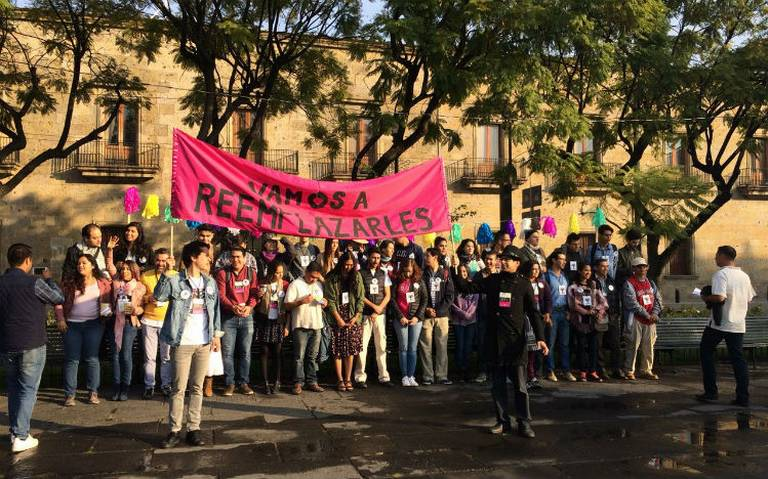
\includegraphics[width=\linewidth]{reemplazarles.jpg}
	\caption{¡Vamos a reemplazarles!}
	\label{fig:reemplazo}
\end{figure}

Para muchas de nosotras era inconcebible que un protopartido pirata se convirtiera en otro partido electorero aunque las personas que lo convirtieron en el fracaso electoral que fue, usaron diversas técnicas de la \hlfix{Ciencia Politica}{¿necesita las mayúsculas?} para conducir a toda la asamblea hacia su propio interés. El cambio de piratas a populistas se explica si pensamos que una organización es un juego con reglas formales e informales. En este caso, las personas más capaces decidieron renunciar a la consigna política que crearon, para usar el poder que les da pertenecer a una élite (familias poderosas, alta educación académica, carisma, estatura, capacidad para hablar, habilidades de negociación o de ciertas jergas populares y agendas consensadas en el movimiento \#YoSoy132) para perseguir su beneficio personal con una justificación mediática suficiente: \emph{somos las personas indignadas que se levantaron en México para denunciar todos los problemas y encontrar todas las soluciones.} Quizá muchas de estas personas ignoraban (y quizá todavía lo hacen) el aura de capital social que les rodea y que las hace prácticamente intocables frente al asedio de corporaciones económicas y partidistas, además de agencias de inteligencia que a lo largo de los últimos sesenta o setenta años se han dedicado a asediar e incluso asesinar a la oposición popular organizada (o sea a las organizaciones sin integrantes de abolengo) en México.

Para quienes nos posicionamos por la pregunta de cómo hacer efectiva y concreta esa otra forma de hacer política, lo primero que aprendimos fue 
\begin{enumerate}
	\item que en México toda forma política es corporativa y está programada en nuestra psique a un nivel \hlfix{casi}{queda mejor decir \emph{prácticamente}.} inconsciente, 
	\item a pensar en los problemas de responsabilidad individual como problemas que se pueden atacar cultivando nuestras potencias, fortaleciendo nuestras capacidades y reconociendo nuestras necesidades.
\end{enumerate}

No creemos en lo que mucha gente dice, que en México la gente es apática y apolítica. El espíritu agachado, arrabalero y huevón de que hablaba la filosofía ---priísta, por cierto--- del mexicano, y que todavía hoy constituye la ideología \emph{whitexican}, es en realidad la abnegación de sabernos sin las armas para combatir, de no querer que nuestras rebeliones no produzcan nada más que muertos y desaparecidos.

Sin embargo, a diferencia de hace unas décadas, hoy estamos en las condiciones tecnológicas para la conformación efectiva de un nuevo poder que cimbre el estado actual de las cosas. Para lograr una transformación real necesitamos accionar desde distintas aristas y facilitando la conexión estratégica entre distintos grupos políticos que buscan abrir y liberar flujos, que aumenten las potencias de las personas. La pregunta pedagógica es:

\begin{quote}
	¿cómo conciliamos todas estas cosas que hemos aprendido desde nuestra experiencia política con acciones articuladas y de gran escala, en diferentes niveles?\todo{Quizá valga la pena en una forma de destacar tipográficamente esto.}
\end{quote}

Hay que darnos cuenta, por ejemplo, de que el rencor contra la partidocracia puede venir inconscientemente de desear el derroche, el exceso y el poder que esa gente tiene. En ese sentido, es importante hacernos \hlfix{la pregunta}{son más de una pregunta, sugiero ponerlo en plural}: si estuviéramos en sus zapatos, ¿cómo crearíamos otras formas de poder? ¿Por qué desearíamos renunciar a nuestros privilegios? ¿Cómo vamos a crear una cultura del encuentro y no del consumo?

La construcción de esta organización política es una metáfora del diseño de una nueva configuración del Estado que permita encontrar un más allá a la catástrofe, que reina a escala micro, \hlfix{molecular}{¿por qué molecular?}, local, y macro, \hlfix{molar}{¿por qué molar?}, \hlfix{global}{¿no será mejor usar el término en español mundial en vez de este falso cognado del inglés?}. Es necesario pensar cómo lidiar con los intereses de actoras individuales, cómo vamos a desarrollar todas nuestras capacidades orientadas hacia un cambio multidimensional, desde dónde lo haremos y cómo conseguiremos recursos.

Estas necesidades se pueden sintetizar, por ejemplo, como infraestructura tecnológica, para innovar con las herramientas que conocemos, gestionadas por \hlfix{geeks}{En cursivas, por ser anglicismo.} por ejemplo; cartografías del poder a través de visualizaciones, organigramas y diagramas de flujo desarrollados por economistas, abogadas y disenadoras; y documentación sobre los protocolos que dan vida a una organización resiliente, a través de procesos y patrones de trabajo.

Así, este texto pretende dar algunas luces a la cuestión de la crisis y la catástrofe, delinear algunos juegos de ficción utópica y posibilidades para empezar a configurar esos territorios imposibles. Desarrollamos algunos síntomas de la crisis política contemporánea, proponemos un modelo para tratar de navegar entre los múltiples factores que causan la opresión de las formas de vida, tanto en su relación con los gobiernos como con sus propios cuerpos. Esta posición escritural es \textbf{La Partida} y podríamos bien señalarla como especulaciones estratégicas, como una corriente de la táctica política. La pregunta central que guiará nuestras reflexiones es \emph{cómo nos organizamos} para un más allá de la catástrofe, cómo creamos un nuevo horizonte. Para nosotras, la estrategia consiste en acciones para visibilizar y combatir las asimetrías de oportunidades y capacidades de las personas y la táctica en configurar prácticas y patrones para las operaciones concretas en el territorio y fuera de él, partiendo del reconocimiento de las circunstancias de cualquier persona que actúa, de cómo en ella se entrecruzan múltiples fuerzas de captura a distintas velocidades.
\chapter{¡Estos son los problemas reales!}
\label{sec:probreals}

\section{El estado actual de las cosas}
\label{sec:stateart}

Aunque \hlfix{usted}{Siento que este recursos de formalidad rompe un poco con el tono usado hasta ahora.} no lo crea, no vivimos por sino a pesar del capitalismo. Se calcula que el ritmo de producción de la \hlfix{economia global}{economia mundial mejor, en español} necesita de aproximadamente \hlfix{cuatro planetas Tierra}{Recuerdo que el dato era de 7.5 para poder vivir de acuerdo al estándar norteamericano.} para ser sostenible.\addref{} La producción de imágenes para capturar el deseo de todas las personas y orientarlos a la acumulación de mercancías a través de la industria cultural nos hace desear el dinero para cumplir con un montón de estereotipos sociales impuestos por la publicidad. ¿Cómo? A través del miedo y la promesa de algún día estar por encima de las demás personas. Mientras, el trabajo se vuelve más precario conforme la optimización y automatización, administrativa y de procesos, se desarrolla en la \hlfix{economia global}{economia mundial mejor, en español}. A los desempleos masivos hay que sumar la incapacidad de los Estados de solventar las deudas sociales, de garantizar algún mínimo de estabilidad o de responder por la gente viviendo en la miseria. Nadie se da cuenta de que se enferma por el cambio climático porque no hay responsables aparentes para la contaminación y deterioro acelerado del planeta y de los recursos disponibles. El \emph{mainstream} tiende a asociar a la enfermedad con el azar o a la voluntad de Dios, una creencia azarosa que solo hace que las personas sigan aguantando las injusticias, para que sigan trabajando y comprando cosas que las hagan sentir valiosas.

A nuestros padres y a algunas personas historiadoras les encanta señalar que el mundo tiene un cauce definido. Sin embargo, saber cómo han sido las cosas en el pasado no significa que estemos condenadas a vivir lo mismo. Reconocer nuestro pasado es el mejor punto de partida para dar forma a un porvenir. Nuestra generación vive cada vez más la tecnología como una cuestión política. La potencia de la piratería y de los movimientos de código abierto (\emph{open source}) son ejemplos de cooperación más allá del mero lucro. Este es un punto de partida que nos da la fuerza para crear un movimiento que nos ayude a ocupar y abrir diferentes espacios. Las personas \emph{millennial} hemos nacido en una tensión histórica. Por un lado, tenemos acceso a un montón de información y un anhelo de libertad que nos impulsa a salir a la calle para encontrar una alternativa al presente. Por el otro, somos presas de la economía de la atención, personas adictas a interacciones virtuales y a códigos publicitarios cada vez más seductores.

\begin{figure}[htbp]
	\centering
	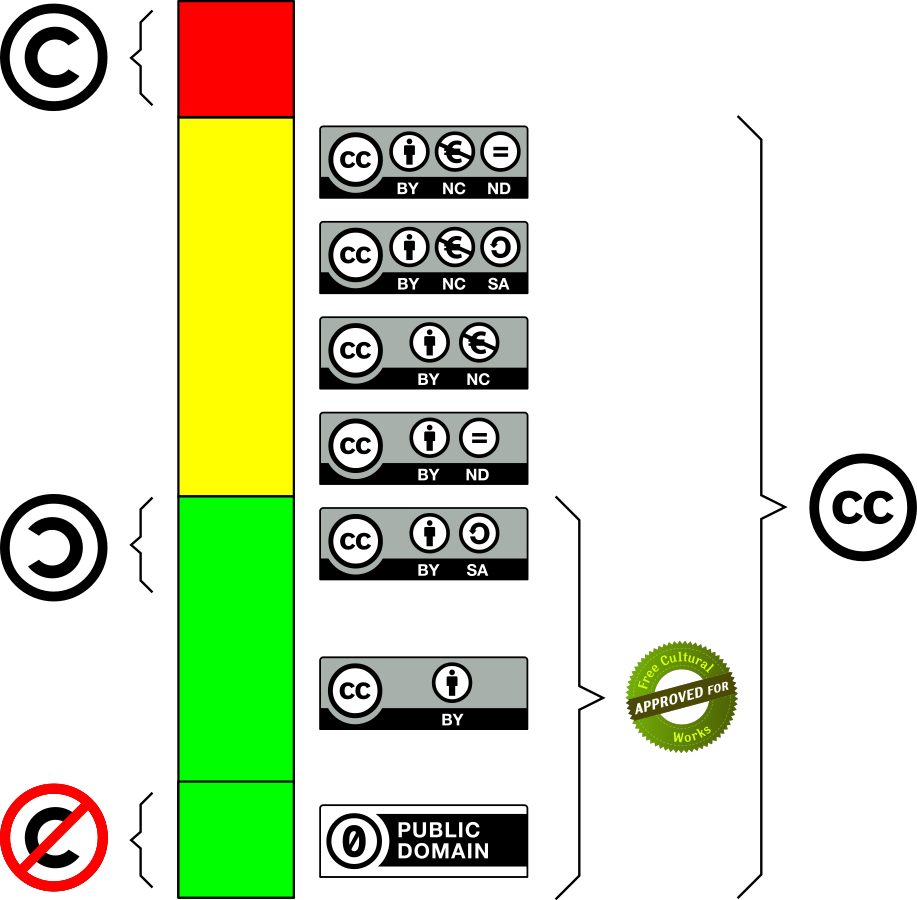
\includegraphics[width=0.8\linewidth]{creative-commons.png}
	\caption{Semáforo de licencias de Creative Commons.}
	\label{fig:CCsignal}
\end{figure}

Aunado a ello, las formas de violencia a las que son sometidas las personas son múltiples y complejas. Una apuesta política transformadora tiene que permitir reconocer estas violencias y dar herramientas para poder combatir. Queremos que todas podamos luchar.

Hay una diferencia abismal entre la violencia total, mutilante, hacia un enemigo abstracto (los criminales, las drogas, \enquote{el enemigo}\revquotes{}) y el roce propio del conflicto en la palabra, a través del habla y la escucha, mucho más vital y espontáneo, donde somos cuerpos que resuenan, que se transmiten. El problema es que nos enseñan que la violencia física, el poder del Estado, es la única manera de lidiar con nuestras diferencias, con nuestros deseos y con el desacuerdo. Para una transformación real, tenemos que \hlfix{hacer ingenieria inversa la caja negra}{O dices \emph{hacerle ingenieria inversa a la caja negra} o \emph{hacer ingenieria inversa a la caja negra}} y tratar de entender cómo se configuran las relaciones de poder y las reglas que dan sentido al Estado. Vivimos en una era en la que, con internet, robots y un sinfín de tecnologías, es técnicamente posible hacerlo. Se trata de permitir que todas las personas seamos co-creadoras de la realidad, que seamos potentes.

\section{Wikipolítica, ¿partido?}
\label{sec:wikipartido}

En 2018, Wikipolítica apostó todo por ocupar el Poder Legislativo en diversos estados de la República mexicana. Si bien no negamos que este es un paso necesario para proyectos de cabildeo estratégico, al no tener una visión de largo plazo, es decir, un programa de gobierno, nuestro experimento creó una red de voluntarias para salir calle a costa de reproducir las mismas dinámicas de explotación que cualquier trabajo o forma de activismo tradicional. Nos encontramos frente a un problema muy grave porque la energía de todas las personas decayó con nuestra terrible derrota en la contienda.

Frente a ello, la respuesta de algunas personas ha sido iniciar otro aparatoso e incierto proceso para crear un partido electoral. Desafortunadamente, el contexto del país es apremiante y la burocracia electoral es un camino de picar piedra. Vivimos una guerra que ha dejado cientos de miles de personas muertas y desaparecidas. Esto nos obliga a pensar en una alternativa radical al modelo extractivista, dependiente de los capitales financieros internacionales. Para muchas de nosotras esta guerra es invisible, pues, en efecto, es difícil reconocer que vivimos en una guerra por la fortuna de vivir en zonas seguras que están lejos de las huellas de la pobreza y la miseria, ya sea en otro país, en otra ciudad o simplemente en otro barrio. Nuestra incapacidad de verlo no significa que la crisis sistemática de derechos humanos, el exterminio feminicida, el auge del totalitarismo tradicionalista y el creciente poder de los capitales extranjeros no exista o vaya a terminar por sí solo.

La situación de nuestro país nos coloca frente a un problema de asimetrías de poder muy claro. Aunado a eso, desde 2016 este país se encuentra en un Estado de excepción. El despliegue y la militarización de las fuerzas del orden tienen como propósito hacerse del control territorial que el narco ha arrebatado al Estado mexicano, pero también para identificar, vigilar y repeler con hostilidad mortal a quien se oponga a los reptiles que pagan a las corporaciones armadas para velar por sus intereses.

  
\begin{figure}[htbp]
	\centering
	
\includegraphics[width=.9\linewidth]{reptilianos.png}
	\caption[Reptilianos conspirando.]{Reptilianos conspirando. Mira \enquote{Lo malo del capitalismo} en ContraPoints de YouTube.}
	\label{fig:reptilianos}
\end{figure}

Ya, en serio, los reptilianos quizá no sean lagartos pero sí agentes de la utilidad, del plusvalor, es el 1~\% que siempre están buscando especular con su dinero para generar más dinero, a costa de quien sea y de cualquier daño al ambiente.

Volviendo al tema, la idea de un Partido meramente electoral es poco eficiente y bastante proclive al corporativismo patriarcal. Muchos machos adeptos a la disciplina del Partido hegemónico son también virilistas, amantes de la disciplina y el sometimiento al falo (al sacerdote, al patriarca), de la camaradería \emph{buenaondita} que invisibiliza las incapacidades de quienes asumen el papel de soldado \hlfix{razo}{Es \emph{raso} en realidad.} en un ejército de activistas. Como si de la disciplina y el control fuese posible producir otra cosa que no sea represión y esquizofrenia.

La historia no tiene un motor y cada cambio lleva consigo una posición sobre el presente, sobre el ahora. Lo único que nos permite creer en nuestra posición como \emph{La Partida} es la tecnocrítica, que significa que a cada instante nos cuestionamos cómo hacer cosas efectivas. Recuerden que la pregunta que nos hace pensar en el porvenir es cómo nos organizamos estratégicamente sobre los problemas estructurales que originan más formas de violencia. Si no pensamos así, seguimos en una cultura de la inmediatez que niega la magnitud y complejidad del problema, que sigue la corriente de los medios de señalar que no hay alternativas sistemáticas que nos muestren imágenes de otra sociedad.

Nos encanta la posición feminista que no encuentra sentido en la necedad electoral y en el deseo de Estado que late en la representación política. Nos parece que más allá de conquistar la hegemonía sobre \hlfix{UN}{hay que resaltarlo tal vez de otro modo} sentido común, se trata de crear canales por donde naveguen ríos de una multiplicidad de sentidos. Para nosotras, se trata de ir más allá de la vieja dicotomía izquierda y derecha.\todo{Sin caer en falsas dicotomías como la que muestra el diagrama de Nolan, por ejemplo.} No queremos representar a nadie, ni gobernar, pero sí que nos preocupa la representación y el gobierno. Queremos que la gente recupere su propia voz, que ella misma pueda defender sus batallas, no queremos más paternalismos. Compartimos la lucha de la gente que pugna por una libertad radical, queremos dar voz, pero no partimos del dolor, partimos de la alegría y de la tecnocrítica como fe práctica, como creencia en la acción. Queremos que la gente pueda gobernarse maximizando la eficiencia de sus recursos y brindándoles nuevas herramientas. Sentimos que se trata de \hlfix{resetear}{Mejor decirlo en buen español: reiniciar} los símbolos culturales que existen alrededor de las herramientas que nos permiten gestionarnos. A lo largo de estos años, nos hemos dado cuenta de que es muy probable que las cosas que \hlfix{se te ocurran}{Contradicción con el tono usado al principio del capítulo que aparece en la primera nota del mismo.} para hacer un cambio suenen demasiado obvias, o sean muy difíciles o ya existan. En ese sentido, creemos que la tarea está en descubrir cómo hacerlas fáciles o que, si existen, sean conocidas por la gente que quieres que lo conozca, es decir, en crear una práctica de \emph{mainstreaming politics} (políticas sobre canales masivos).\footnote{Hemos pensado en estas prácticas como transversalización, basado en el criterio de la ONU sobre \emph{gender mainstream}.}\addref{}

\section{¿Qué tan efectivo es el activismo?}
\label{sec:activismo}

\begin{figure}[htbp]
	\centering
	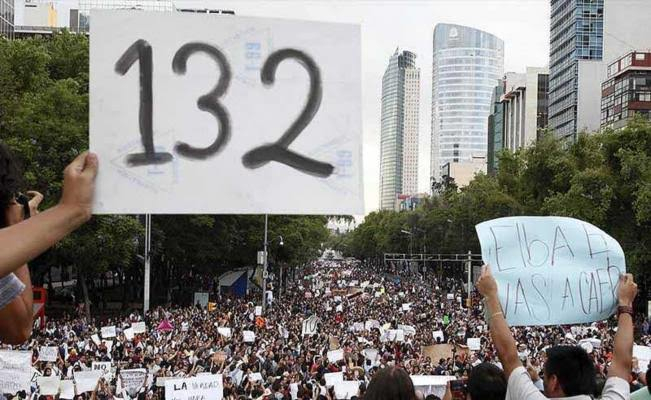
\includegraphics[width=.9\linewidth]{132.jpg}
	\caption{Asambleítis.}
	\todo[inline]{Mejorar la leyenda de la figura.}
	\label{fig:132}
\end{figure}

Los análisis de muchos activistas intelectuales de izquierda presuponen conspiraciones globales elaboradas, como si la estupidez global contemporánea fuera algo planeado. Ni siquiera los reptilianos en sus reuniones en Davos piensan en controlar al mundo. La modernidad es un discurso al cual aferrarse cuando en verdad el Medioevo nunca acabó. La aristocracia, la burguesía, la gente en el poder, son solo idiotas a quienes les gusta tener pisos de mármol, comer en restaurantes caros, vestir ropas caras y mirar sus números crecer.

\begin{quote}
	La verdadera tragedia del presente es lo que alguien llamaba la \emph{banalidad del mal}.\addref{}
\end{quote}

Mientras, nosotras vemos que el problema más grave que enfrentan las resistencias de calle es \emph{articularse} con otros esfuerzos. Muchas redes de movimientos de base, de activistas defensores de DD.HH., etc., tienen que trabajar con la sociedad civil, otra casta de aristoburguesía que actúa desde una clase privilegiada. Aunque no lo parezca, incluso en las resistencias pervive la lucha de clases.

A veces parece que entre las personas activas políticamente prevalece una atmósfera de rectitud moral, como si fuera evidente que lo que están haciendo para tratar de cambiar el estado de las cosas es lo correcto. En términos prácticos, resulta poco atinado querer imponernos frente a la gente, tomar nuestra visión política como algo evidente, con un vocabulario cerrado, cuando es una cosmovisión de clase (es decir, condicionada por nuestros hábitos de consumo y poder adquisitivo). La lucha es más eficiente entre más aprendemos a compartir, a socializar, a hacer un ejercicio mayéutico que le permita a la banda darse cuenta por ella misma de lo que quieres hacerle ver.

En este sentido, la militancia requiere aprender a escuchar a las personas para tener una aproximación más o menos clara de sus creencias para entender que la persuasión está en la apertura misma al diálogo. Después de todo, la libertad sólo existe en el momento en que somos capaces de tomar una decisión, y la lucha política es una decisión, nunca es evidente. Para empatizar, una tiene que posicionarse con \hlfix{ternura radical}{¿es esto un concepto acaso?} frente al otro. Hay que tener presente que las cosas que otras personas hacen tienen sentido de algún modo, al menos para ellas. En pocas palabras, no hay ninguna forma de vida que sea intrínsecamente más valiosa que otra. La clave está en reconocer los afectos como parte de la racionalidad política.

Mientras tanto, las personas afines al liberalismo (a la \hlfix{buenaonda}{en cursivas}, a la omisión del conflicto, a quienes reconocen que la única posibilidad es institucional) se retuercen frente a un momento de posverdad y de noticias falsas. No se explican qué llevó al mundo a semejante \enquote{irracionalidad},\revquotes{} no entienden que jamás la hubo y que los síntomas contemporáneos son también una oportunidad de crear un nuevo horizonte político. En medio de la crisis que vivimos diariamente, nuestra experiencia de la realidad como flujos de información (\emph{links, chats, shares}\ldots{}) nos da una capacidad que antes era imposible, para producir efectos en el mundo. Pero nuestra generación sufre porque somos conscientes del cinismo ilustrado que prevalece en el espíritu universitario, porque sabemos que tenemos el potencial técnico para vivir un mundo abierto, libre, pero no sabemos cómo (¿o realmente no queremos?) crearlo.

Nuestra visión de la estrategia simpatiza con una corriente conocida como xenofeminismo interseccional\addref{} y considera que las subjetividades están atravesadas por el género y por otras categorías que causan opresión en distintas dimensiones. La novedad radica en concebir estas categorías como dispositivos, es decir, como tecnologías que han sido diseñadas por alguien con fines en particular. El costo de nuestros fracasos al momento de actuar políticamente no es solo organizacional. Se trata, ni más ni menos que de una complicidad con el deterioro ecológico y la violencia interseccional (cuyo punto de culminación es la muerte) sobre las formas de vida, además del perfeccionamiento incesante y los procesos interactivos del parásito capitalista.

\begin{figure}[htbp]
	\centering
	
\includegraphics[width=0.6\linewidth]{xf.jpg}
	\caption{}
	\todo[inline]{Agregar una leyenda a la figura.}
	\label{fig:xf}
\end{figure}

\section{El cinismo es otra estrategia}
\label{sec:cinismo}

Hemos visto con tristeza que muchos movimientos políticos cargan con la melancolía de los vencidos, un estado de ánimo muy común a las izquierdas. Los hombres que lideran usualmente dan la apariencia del príncipe bucólico y carismático, como arquetipos del Che Guevara o de otros guerrilleros revolucionarios. A veces parece que el folclore que forman entre los grupos obedece más a su necesidad de sentirse abrazados por una comunidad de seguidores, a su incapacidad de superar sus traumas familiares o simplemente a cosas muy básicas como impulsos de destrucción o de tener sexo. Hemos visto muy pocas personas con un deseo genuino de crear una alternativa real, de actuar estratégicamente. Como lo vemos, los líderes machos se entregan al cinismo porque les es más cómodo usar la razón como instrumento para su beneficio. Estas personas se convierten en ideólogas, argumentan siempre en favor de lo que les conviene. Su postura es anacrónica, es decir, que no considera la evolución histórica ni las coyunturas que dan forma a las sociedades a través del tiempo, mucho menos considera que vivimos en una sociedad extremadamente compleja donde el capitalismo se manifiesta a través de algoritmos e instrucciones programadas en los comportamientos de las personas. Hay una estrecha relación entre esta posición de comodidad, de desvarío y de hipocresía irónica, y la crisis de fe contemporánea que hay que enfrentar para poder construir una alternativa. Por supuesto, el cínico reprimirá estos síntomas para seguir gozando de los beneficios materiales de hacerse pendejo, al costo de invisibilizar un montón de normas violentas necesarias para afirmar su identidad de macho ilustrado. Pero su posición significa varias cosas.

\begin{quote}
	Nota mental: \emph{El patriarcado no tiene género}.
\end{quote}

Por una parte, es la muestra de que vivimos un profundo vacío espiritual que necesitamos entender a través de sus síntomas para lograr crear una alternativa a la religión del Yo. Así como la teología de la liberación sirvió en su momento para la articulación política de subjetividades despojadas de su tierra, hoy necesitamos crear una nueva teología pop que haga frente a la falsa conciencia ilustrada contemporánea, que plantee un horizonte hacia la libertad a través de diferentes visiones religiosas, traduciendo ideas a través de significantes equivalentes.

\begin{figure}[htbp]
	\centering
	
\includegraphics[scale=1]{century.jpg}
	\caption[\emph{The Century of the Self}]{El documental \emph{The Century of the Self} de Adam Curtis trata sobre cómo nació esa religión del yo.}
	\todo[inline]{Mejorar la resolución de la imagen.}
	\label{fig:century}
\end{figure}

Por otro lado, el peligro de estos hombres representantes es que su aliento heroico parece ignorar que vivimos en una guerra y que es absolutamente imprescindible tomar posición por acciones estratégicas que ataquen transversalmente varios problemas. Necesitamos entender que la evolución del capitalismo de \enquote{modo de producción}\revquotes{} a \enquote{modo de consumo}\revquotes{} y el paradigma de informatización de la economía, rompieron con la articulación de movimientos de clase, al estructurar la sociedad de tal modo que la identidad se configura a través de las mercancías consumidas y no de los vínculos afectivos entre personas. Accionar hoy requiere ser consciente de la lógica de la dominación contemporánea y no solo de las instancias tradicionales de incidencia.

\subsection{\emph{La verdad} es un instrumento}
\label{sub:verdadinstrumental}

\begin{quote}
	Hoy parece más fácil imaginar el fin del mundo que el fin del
	capitalismo.\\ \emph{Fredric Jameson}.\todo{¿Es un epígrafe esto}
\end{quote}

El mundo no se acaba, se acaban las sociedades. Específicamente, se acaban quienes padecen las sociedades. Se acaba el hábitat de quienes solo tienen la tierra. La ecocatástrofe es la tragedia del exterminio de quienes viven en el margen, en las periferias. No es una lucha por la conservación del planeta sino por la vida de quienes padecen los residuos contaminantes del capitalismo. En medio de esta ecocatástrofe, la noción de \emph{verdad} tiene sentido para pensar en cómo se configura la memoria y la validez de los argumentos para un grupo de personas en particular. La verdad es el filtro con el que se mira, aquello que se considera valioso. Está relacionada con el recuerdo y está mediada a través del lenguaje, que articula nuestras experiencias en imágenes. La verdad siempre es a través de un observador, la verdad nunca está en el acto. En el acto hay presencia, realidad.

\begin{figure}[htbp]
	\centering
	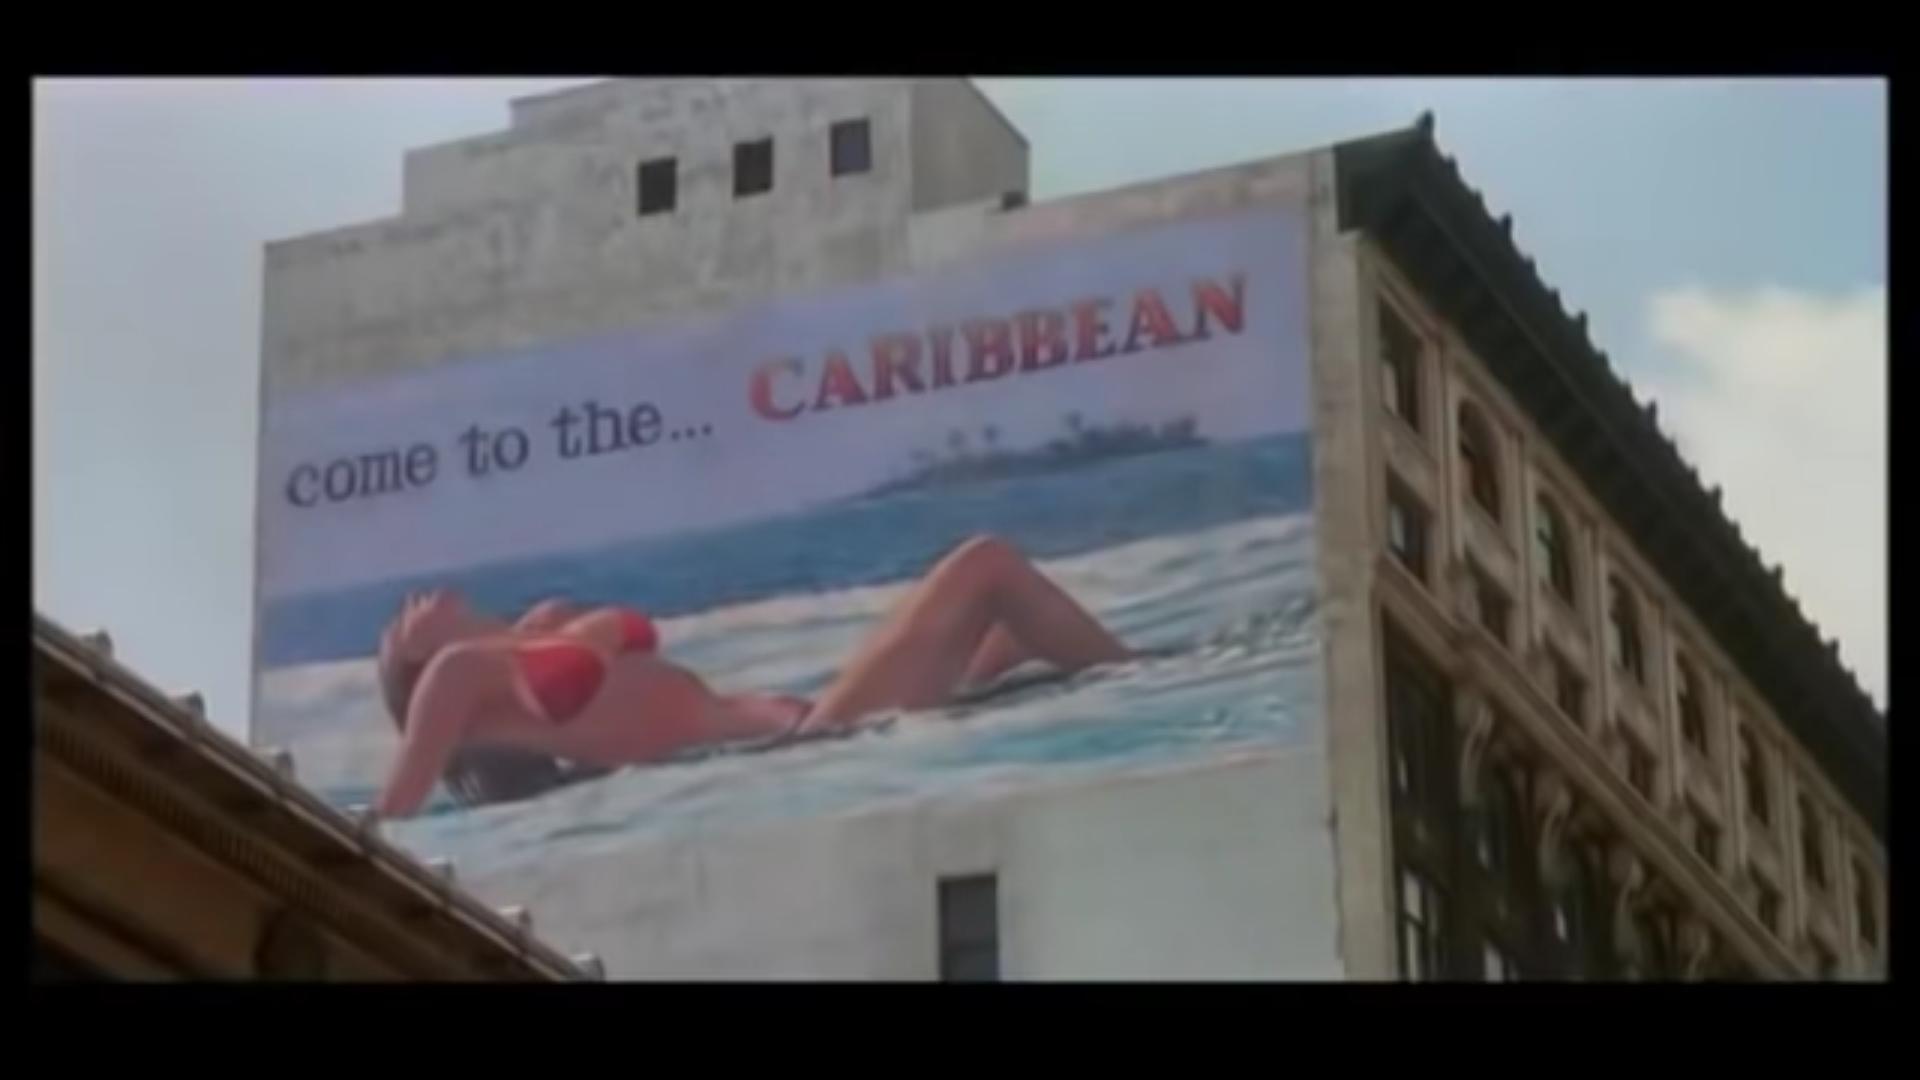
\includegraphics[width=.9\linewidth]{images/ideology1.png}
	\caption[Anuncio sin filtro.]{Anuncio sin filtro. De Slavoj Žižek en el documental \enquote{The Pervert's Guide to Ideology}}
\end{figure}

\begin{figure}[htbp]
	\centering
	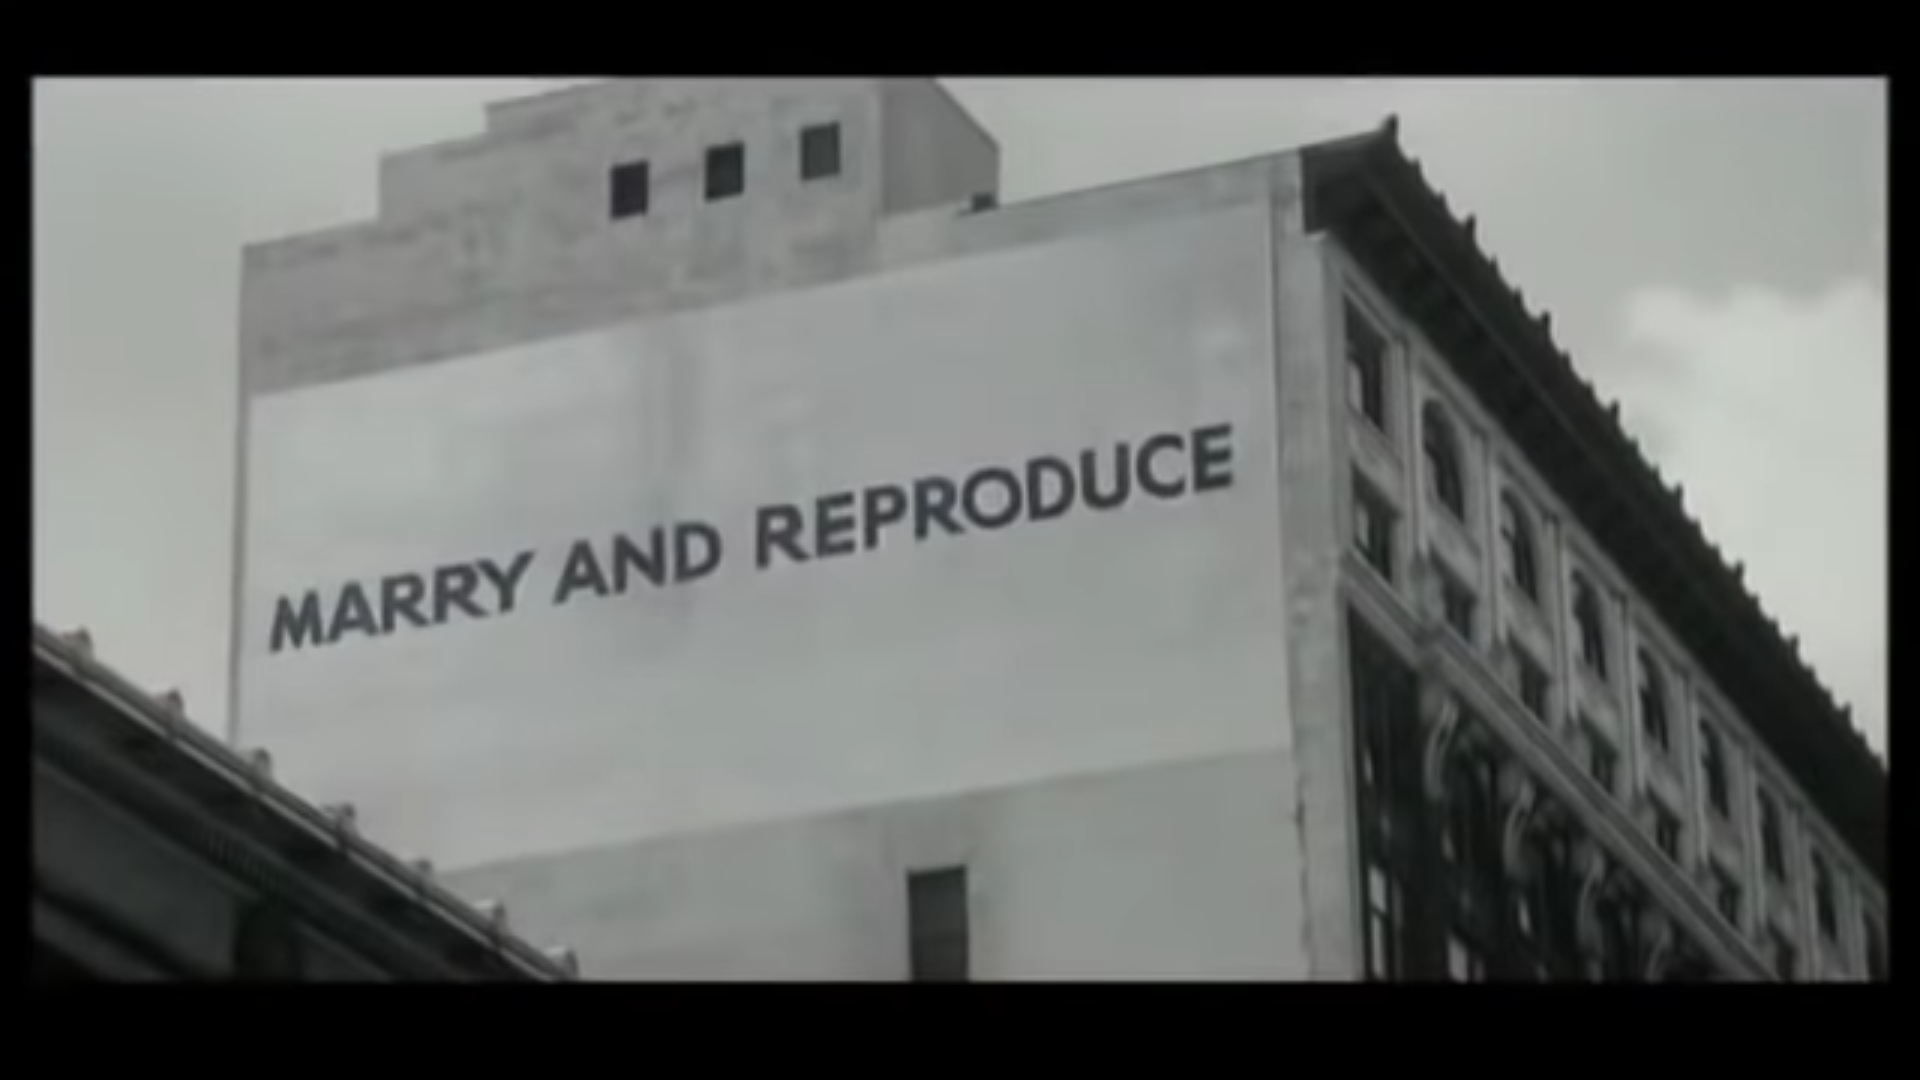
\includegraphics[width=.9\linewidth]{images/ideology2.png}
	\caption[Anuncio con filtro.]{Anuncio con filtro. De Slavoj Žižek en el documental \enquote{The Pervert's Guide to Ideology}}
\end{figure}

La noción de \enquote{conocimiento} proviene de una tradición de pensamiento que ignora otro tipo de \emph{saberes}, como la sensibilidad artística, la salud\footnote{Salud como buen vivir, por encima de la concepción que define la salud en sentido negativo, como ausencia de enfermedad, como lo mínimo necesario para que las personas estén aptas para producir. \url{https://www.theguardian.com/sustainable-business/blog/buen-vivir-philosophy-south-america-eduardo-gudynas}} o la relación con la tierra, la memoria y la conciencia sobre el territorio. Una militancia crítica, efectiva y consciente requiere la capacidad de comprender cómo se configuran los procesos históricos, testimonios y experiencias, de personas que hablan desde el lugar que habitan y cómo esa relación configura una identidad, no desde la historia oficial, de sucesiones de reyes y héroes grandiosos. Para lograrlo, es necesario renunciar a las pretensiones de verdad absoluta y a la culpa producida por la cultura del \emph{deber ser}. No hay una verdad por la cual luchar, hay verdades situadas según intereses. La tecnociencia es una herramienta transformadora, que puede servir para terminar con la escasez de alimento tanto como para perfeccionar un ejército. Es necesario asumir una posición en la que nada es evidente y todo acontece en la apariencia, obligándonos a estar atentas a nuestros juicios. El xenofeminismo nos permitió bosquejarlo como algo parecido a una pedagogía de la complejidad del mundo, que requiere una actitud casi estoica, contemplativa, de aceptación que hay que tener frente al mundo, como una postura de diálogo con la alteridad, con todo aquello que no es lo que creemos que somos nosotras individualmente.

La derecha alternativa (\emph{alt-right}) ha sabido bien utilizar la verdad como un arma. Dentro de este movimiento se critica mucho la idea de que la izquierda vive en una Catedral, haciendo alusión a una política dogmática y sectaria. Sabemos que esta postura no es otra cosa sino el partido del resentimiento total pero son, al mismo tiempo, tan básicos que nos han dado una buena idea, la de crear espacios como las Iglesias lo son para sus adeptos, pero para que las personas podamos hablar con libertad y recuperar vínculos entre nosotras. Si la derecha se vale de artimañas pos-ideológicas y adopta posturas económicas de la socialdemocracia keynesiana, nada nos impide reconocer que la justificación sobre el uso de determinada estrategia se construye después de que se ha obtenido una victoria. Por eso, si no pensamos en abrir las élites, en infiltrarnos, nuestro poder se verá reducido cada vez más. Las élites detentan el dominio material frente a los oprimidos a través de tecnologías como los códigos culturales del género, la raza o la clase. Sabemos que otras resistencias de izquierda más radical no han podido mantener un impacto, pero sí tecnologías de lucha avanzadas, como procesos, metodologías y códigos de programación que han resultado de distintas luchas de autogestión. No subestimemos sus esfuerzos. Estamos aquí porque hubo un Atenco, hubo una \emph{otra campaña}, hubo un Syriza. Esas luchas tienen que lidiar con el enemigo, quien en todo momento busca despojarle de su terreno, del patrimonio natural o de la vida misma. Ellas nos han enseñado que la autogestión no significa informalidad. Significa comprometernos a cultivar y entrelazar los saberes necesarios para que la gente pueda organizarse autónomamente con sus locales, con quienes comparte una vida común.

Sin embargo, la velocidad con la que la catástrofe ambiental y el cambio de lógicas de segregación a lógicas de gentrificación como forma de exterminio, devoran cada espacio donde es posible vivir, nos obliga a desarrollar tecnologías a gran escala que permitan conectar las resistencias locales a plataformas globales, con el propósito de atacar transversalmente estos problemas. Por ello creemos en una política de muchos frentes, multilateral, estoica y pragmática. Desde la izquierda y la derecha, desde arriba y desde abajo.

Hay que recordar, sin embargo, que muchas resistencias provienen de organización popular frente a los desplazamientos forzados por megaproyectos y otras imposiciones estatales. Frente a estas necesidades, es prioritario que pensemos el activismo político tratando de articular proyectos, siempre desde el territorio, creando vínculos comunes con gente que comparte agendas, o fungiendo como líderes comunitarias para resolver algún problema en común con los vecinos. Es decir, crear una base social de simpatizantes a través de la participación real en la comunidad. Una buena forma de hacer esto es, por ejemplo, analizando el código (los memes) que configuran una experiencia concreta de lo real para un grupo de personas y crear imágenes que la gente haga suyas sobre cómo organizarse, cómo participar desde su circunstancia particular, partiendo de comprender las motivaciones y necesidades de las personas. Saul Alinsky, un organizador comunitario muy importante en Estados Unidos durante la primera mitad del siglo XX, insiste en tener una ética basada en principios interpretables, no universales sino en tensión. A grandes rasgos, esto significa jugar un rol de mediador a través del reconocimiento de las diferencias y con entrenamiento para crear consensos y resolver disputas. Pero, sobre todo, reconocer que el \emph{trabajo} y la forma en que \emph{deseamos} son cuestiones clave para encontrar una alternativa a la crisis.

\section{Un trabajo político efectivo}
\label{sec:org0d34f13}

En términos concretos, necesitamos aprender a trabajar en calidad de iguales, a escucharnos y a delegar. La tarea es compleja y requiere acciones multidimensionales, desde distintos frentes. Por ejemplo, frente al panorama mundial, necesitamos dialogar con distintos movimientos alrededor del planeta, desarrollar una política internacional que podamos empujar y difundir en la opinión pública, abrir líneas de estudio y tender puentes con los diferentes sectores con los que estemos presentes. No necesitamos ser protagonistas de la lucha, como lo demandaría la ideología de la representación política, sólo crear las condiciones de posibilidad para que suceda. A esto nos referimos con la idea de abrir espacios para que todas podamos ocuparlos. Tenemos que ser estratégicas y usar con precisión herramientas de redes sociales pensando en hacer sexy el activismo/militancia política para más personas. Estas cuestiones nos abren preguntas de comunicación y mercadotecnia como:

\begin{itemize}
	\item ¿cómo nos diseminamos estratégicamente?
	\item ¿con quién queremos crear lazos?
	\item ¿cómo nos hacemos visibles para otras simpatizantes?
\end{itemize}

En función de nuestra capacidad de acercarnos a la gente que nos apoyaría, podemos encontrar alternativas de financiamiento, como la creación de un ecosistema de cooperativas donde las personas puedan ser consumidoras y productoras. Para lograrlo, podemos hacer labor política en nuestras redes para identificar prácticas y proyectos útiles, como los de sistematización de metodologías de organización o lo que ayude a que todo sea más democrático y eficiente.

La cuestión está en tratar de que todo lo común a nosotras (espacios, recursos, expresiones) tengan mecanismos efectivos de implementación local, que cualquier persona pueda acceder a nuestros recursos y organizarse. Esto es posible con una pedagogía de organización personal y comunitaria a partir de hábitos y prácticas. No se trata de compartir un canon ilustrado sino de descubrirse como manifestaciones concretas de la humanidad y trabajar entre todas para vivir alegres. Para ello tenemos que plantear del principio de que las organizaciones se planean y diseñan desde sus usuarias y desde sus operadoras. Esto significa que nuestros procesos también deben estar diseñados para \emph{nosotras, las personas} que los operamos. Con la intención de ser siempre una organización diseñada para la hospitalidad, para atraer la atención de todo el mundo y poder acercarle una vía para interactuar con la organización y participar políticamente desde su circunstancia.

\begin{figure}[htbp]
	\centering
	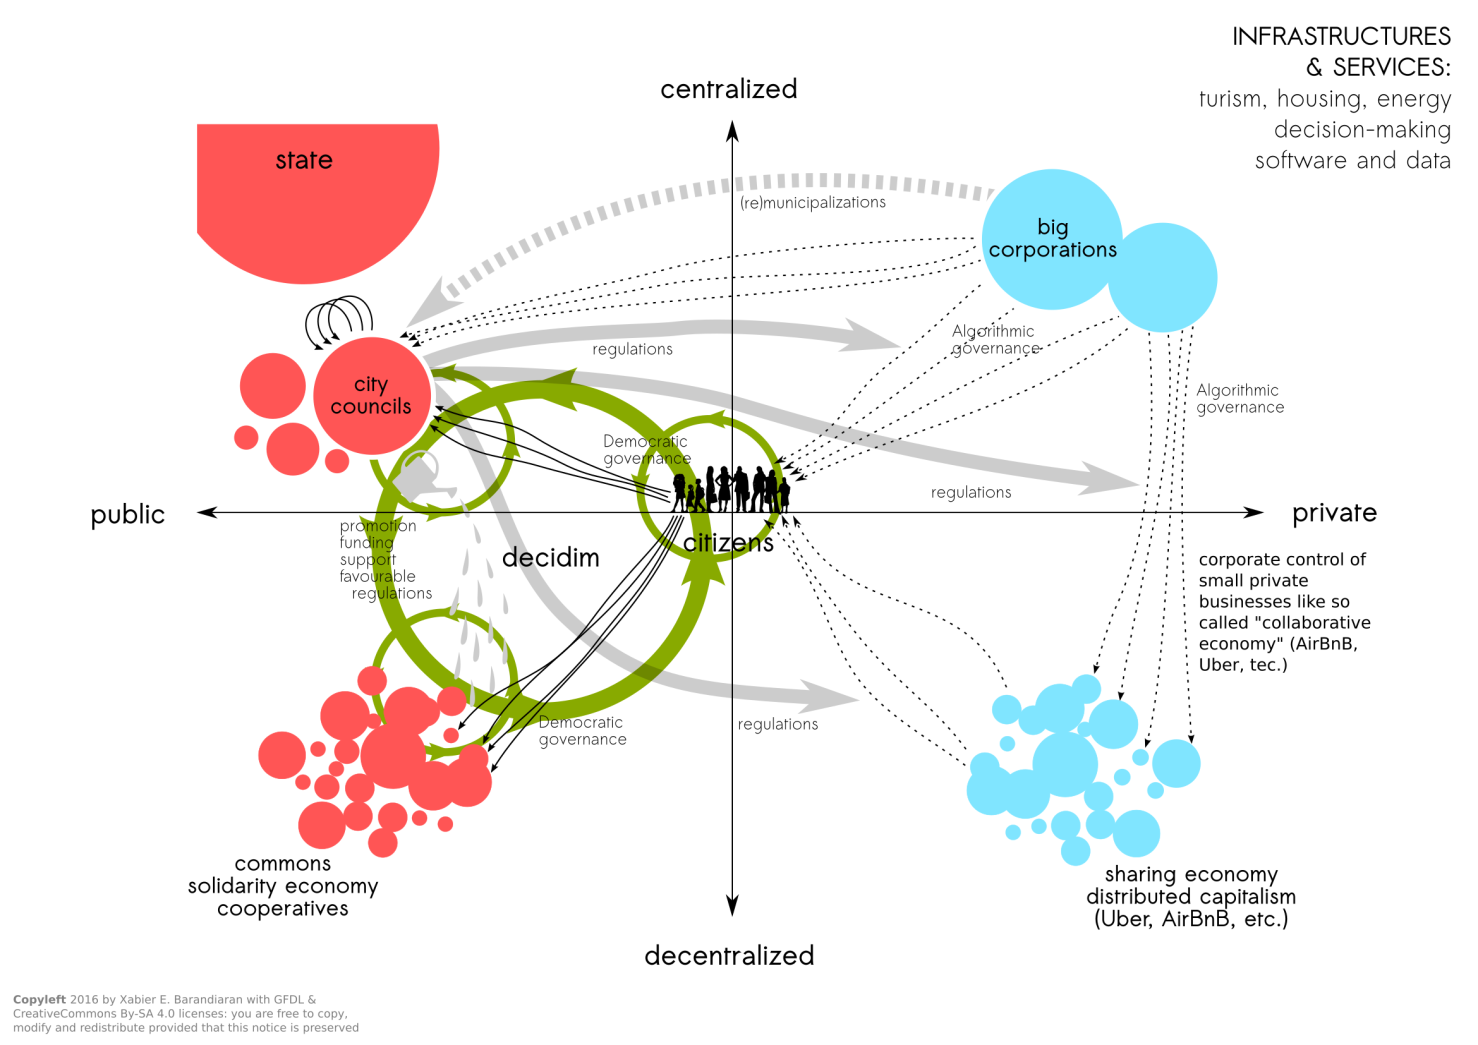
\includegraphics[width=.9\linewidth]{decidim-context.png}
	\caption[Proyecto Decidim.]{Un ejemplo de formas de organización social y el aporte del proyecto Decidim.}
	\label{fig:decidim}
\end{figure}

También necesitamos procedimientos de creación colectiva.\footnote{El proyecto \url{decidim.org} es un buen ejemplo de plataformas de organización colectiva.} Crear dinámicas, herramientas y saberes comunes, además de hacer un reconocimiento explícito de posturas ideológicas para que cada grupo pueda desarrollar su agenda y así crear un plan de trabajo global donde cada representación temática se encargue de desarrollar su agenda. En este sentido, vemos al liderazgo como encuentro y mediación que necesita que desarrollemos tecnologías de la presencia para diseñar espacios donde se pueda gestionar adecuadamente el conflicto. Se trata de construir desde nuestras diferencias y no a pesar de ellas, de reconocer que los qués se resuelven en los cómos, es decir, que los grandes conceptos abstractos se vuelven tangibles a partir de los detalles de implementación. Hay tribus donde los jefes de tribu son únicamente las personas que consultan y toda su autoridad se basa en opinar la manera más acertada de hacer algo sobre lo que deciden en concreto las personas que saben cómo hacerlo. Sería bueno que cada persona que integra una organización supiera un conjunto de habilidades mínimas, como liderazgo, comunicación, gestión del trabajo o programación, para poder crear equipos realmente transdiciplinarios ajenos a la necesidad de tener la razón, de tener \emph{la verdad}.

\section{¿Cómo crear una alternativa?}
\label{sec:alternativa}

El deseo de Estado es realmente el problema que más nos preocupa, por eso pensamos que la crisis de nuestro tiempo es una crisis de la imagen. A grandes rasgos, el deseo opera como una respuesta activa de nuestra psique a la impresión que las imágenes producen en nuestros cuerpos. El Estado reproduce el Patriarcado y funciona de maneras muy sutiles, desarrollando tecnologías que transforman nuestro deseo en un canal para la transmisión de mercancías, para que nuestras respuestas sexuales sean capitalizables como grandes masas de tráfico de información. Si la sensibilidad ha sido durante mucho tiempo una mera disposición pasiva al sufrimiento, ahora tiene que volverse el medio mismo del combate, ser una ciencia de la transmisión de imágenes y del hackeo de significados, ser la ciencia de los memes. El arte político de redirigir el sufrimiento en fuerza, el odio hacia uno mismo y los impulsos de autosabotaje en rabia hacia las normas impuestas por el mundo exterior, y la desesperanza en coraje para luchar por seguirnos encontrando y construyendo, aunque a veces sea difícil. Tenemos que aprender a reconocer nuestros deseos y a hackear el resentimiento de clase,\footnote{El resentimiento de clase es, por ejemplo, la envidia que te produce tener que usar transporte público todos los días y estar expuesta a asaltos mientras que la persona de al lado, o de la otra colonia, viaja con chofer privado en un automóvil particular.} así como darnos cuenta de nuestros privilegios y de la importancia de nuestra historia y de nuestra clase para la organización política.

La maquinaria estatal se encarga de orientar todas nuestras voluntades a proyectos que sirvan para construir un orden donde todas las personas son ciudadanas, sí, pero también son soldadas, consumidoras y espectadoras de lo que es producido como lo real. Necesitamos pensar el modo de generar un sentimiento de creación que no se sienta como el sentimiento de los débiles de la izquierda, que no se sienta como revolución permanente sino como un mundo nuevo que surge de las cenizas pero no tiene el martirio de la filosofía existencialista porque es un sentir comunitario, porque no tiene la característica del abandono que veían esos filósofos individualistas, un mundo que está vivo y presente, alegre.

Una verdadera alternativa es la creación de un nuevo poder, de comenzar a construir un mundo donde efectivamente quepan muchos mundos. Desde el contexto político latinoamericano, la construcción de un proyecto de país es parte de lo que llamamos \emph{poder constituyente}, una articulación política para un nuevo contrato social. Una coalición de fuerzas progresistas para una agenda de innovación estratégica cuyo fin sea hacer efectivo el buen vivir o bienestar para todas las personas. Esta multitud se articularía alrededor de agendas, sectores y esferas de acción basadas en recursos comunes y en la visión FLOS (\emph{free, libre and open sources}), un concepto que desarrollaremos más adelante. Esto significa desarrollar una base social a través de una plataforma que permita que la gente se organice, un imaginario común del futuro y un repositorio de tecnologías que permitan a la gente \emph{saber hacer}.
\setchapterpreamble[u]{%
	\dictum[Christiane Taubira refiriéndose al presidente Macron.]{Los fracasos políticos son temporales, pero las derrotas semánticas y
	culturales son dramáticas porque tardan más en revertirse.}
	}
\chapter{Lee esto antes de \emph{hacer} algo}
\label{cha:antesalgo}

El nuestro es un mundo de redes, navegable a través de teorías de la complejidad y del caos. Muchos procesos automáticos alimentan diariamente el flujo de operaciones de las infraestructuras (redes de abasto de combustibles, electricidad para servidores, satélites, líneas de internet) sin que haya realmente un responsable. Las funciones están programadas y los destinos predeterminados. Miles de variables interactuando entre ellas a partir de distintos nodos que envían información diversa y que demandan u ofertan certificados, \emph{requests}. La idea de la cibernética es dispersar para crear un caos gestionable, incluso automatizable.

\begin{figure}[htbp]
	\centering
	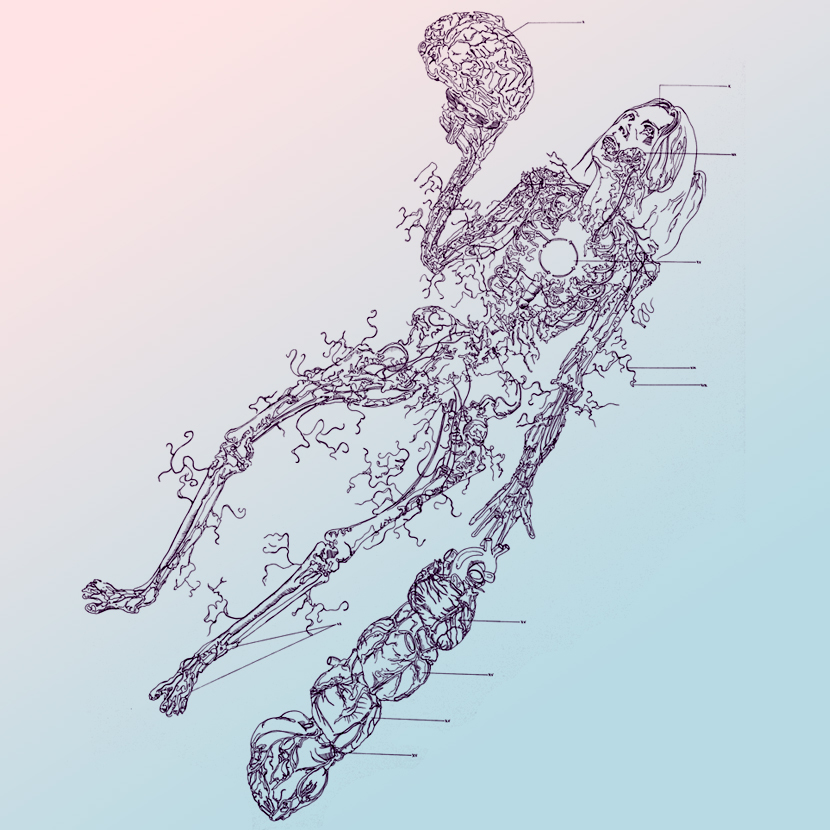
\includegraphics[width=\linewidth]{zombie.jpg}
	\caption{¿Cyborg o zombi?}
	\label{fig:cyberzombie}
\end{figure}

Al mismo tiempo tenemos lo necesario para implementar una economía \hlfix{posescasez}{Me parece que es más correcto escribir \emph{postescasez}.},\footnote{\url{es.wikipedia.org/wiki/Economía\_post-escasez}} sólo se trata de intervenir estratégicamente en esas redes de información, que también son flujos de sentido, producciones de deseo. La utopía robótica es una de las aristas de distintos escenarios posibles planteados por el texto de Peter Frese titulado \emph{Four Futures}, donde señala que viviremos en un mundo materialmente condicionado por dos aristas, una de igualitarismo-estamentalismo (o sea, donde las jerarquías manden) y otra de abundancia (por la automatización tecnológica) o escasez (por nuevas formas de los patrones para crear valor explotable). De esos casos, los más extremos parecen ser el mundo donde quepan todos los mundos, sostenido por una infraestructura tecnológica común, y el exterminio, que es prácticamente lo mismo pero solo para 1~\% de la población global.\footnote{A ello habría que sumar el problema del deseo, pensar en los desarrollos cibernéticos de las economías libidinales o economías del deseo.}

\begin{table}
	\caption{}
	\todo[inline]{Añadir una leyenda a la tabla. Se hizo flotante para poder asignarle una referencia cruzada y vincularla a la sección~\ref{sec:viruscapitalista}, donde se le cita.}
	\label{tab:Aristas}
	\centering

	\begin{tabular}{lll}
		\toprule
		 & \textbf{Abundancia} & \textbf{Escasez}\\
		\midrule
		\textbf{Igualdad} & Comunismo & Socialismo\\
		\textbf{Jerarquía} & Rentismo & Exterminismo\\
		\bottomrule
	\end{tabular}
\end{table}

Según Natalie Wynn\footnote{Famosa por ContraPoints, su vlog en YouTube.}, la derecha de internet pinta una caricatura de la izquierda, con el marxismo posmoderno como la supuesta ideología. Esto es muestra de que una de las operaciones más efectivas del parásito capitalista es poner a pelear a las resistencias en torno a cosas pequeñas y concretas,\footnote{Freud se refiere a esto como el narcisismo de las pequeñas diferencias.} cuando es más aquello en lo que estamos de acuerdo pero tenemos la necesidad de encontrar coherencia teórica en modelos ideales y no en especulaciones sobre la realidad. Esta posición que renuncia a la necesidad de certidumbre intelectual ---es decir, que no va más allá de una pregunta sobre instancias, sobre cómos--- se conoce como realismo especulativo y es cercana a una teoría del conocimiento (y filosofía del ser) llamada \enquote{ontología orientada a objetos}.\revquotes{} Es importante recordar que probablemente las civilizaciones humanas han sido injustas desde el principio de los tiempos, pero la posición que tomamos respecto a la explotación de los patrones, de los propietarios o de los banqueros depende en buena medida de dónde estamos paradas.

Como reza el lema del xenofeminismo:
	
\begin{quote}
	\textsf{\textbf{Si la naturaleza es injusta, ¡cambiémosla!}}
\end{quote}

Podemos hablar desde el arte, generando consensos en torno a acciones comunes en distintos grupos. A veces parece más fácil actuar desde los medios que desde la militancia de izquierda. Nuestras aliadas han repetido ya varias veces la necesidad de hacer un posicionamiento estético sobre el discurso. En nuestros tiempos, en la política rige el principio de que fondo es forma. Y sin embargo, son las cuestiones estructurales como el género, el color de piel, la nacionalidad, el acceso a educación, salud, el dinero, etc, las que más afectan, por una cuestión de origen, de diseño, sobre las tecnologías que configuran nuestra realidad.

Al ser un concepto y no el nombre de un objeto concreto, la influencia del capitalismo se toma por la derecha como un mero principio económico que brinda todas las mercancías necesarias para vivir cómodo. He aquí una de las partes más importantes del problema. Para entenderlo, tenemos que comprender las diferencias entre Estado y Capitalismo en la historia, y cómo funciona a grandes rasgos el espectro político a partir de estas diferencias. Sin embargo, el pensamiento del \emph{status quo} es realmente poderoso pues el Estado dispone de manera muy particular de las armas que reproducen el modo de producción capitalista, las orienta siempre a la eficiencia y optimización que produce valor intercambiable.

\section{¿El enemigo es el capitalismo, el Estado o los mercados?}
\label{sec:enemigos}

Ahora vamos a profundizar en algunas distinciones que sirvan para hacer cosas que generen cambios reales. Sabemos que en este análisis hemos hablado poco del patriarcado pues lo asumimos como parte de la ideología primigenea del capitalismo. Ponga usted mucha atención porque ahí vamos:

El capitalismo, desde una \emph{visión de ingeniero},\didit{se resaltó el término} se trata básicamente de un modo de producción de bienes materiales. Este modo de hacer cosas parte de factores de producción que tradicionalmente han sido resumidos como tierra, capital y trabajo. El marxismo fue importante porque nos mostró un análisis mucho más extenso del capitalismo, al entenderlo como una configuración de las relaciones sociales a través de los procesos productivos, donde las mercancías tienen un valor por sí mismo y tan poderoso que configuran la identidad misma de las subjetividades.

Para nosotras, además de lo que le aprendimos al marxismo clásico, el capitalismo es un modo de producción pero en este momento de la historia también es una \emph{velocidad sobre los flujos de información}. Para sostener lo anterior, es necesario que comprendamos que el viejo escenario económico donde la fábrica jugaba el rol predominante en la producción de valor ha sido reemplazado por una lógica de trabajo que pulveriza y divide en diferentes espacios la línea de producción, de manera que sea más eficiente y barato producir. Y lo que genera más valor en la economía contemporánea no es ya la mercancía como un objeto físico sino la información que producen las relaciones entre las cosas. A esta era de la economía algunas personas la llaman \emph{posfordismo}\todo{Sugiero cambiar por \emph{postfordismo}.} y entre otras cosas, es más una forma de producción regida por el consumo, es decir, la demanda de bienes, que por la producción, como lo fue en las revoluciones tecnológicas pasadas.

El mercado es un conjunto de transacciones. Es la infraestructura del intercambio mercantil y su acontecer capitalista tiene más que ver más con el cobro del impuesto, origen de la financiarización del valor,\footnote{Garzon Espinosa, Alberto. \enquote{¿Qué es la financiarización?} en \emph{Economía Crítica y Crítica de la Economía}. Disponible en:~\url{www.economiacritica.net/?p=144}.} que con el comercio. El capitalismo es un parásito cultural que paraliza el trabajo y subsume los recursos y hábitats del planeta mientras mercantiliza bienes primarios (\emph{raw materials}) en abstracciones virtuales, a través de una economía del deseo. Se in-corpora (es decir, configura una respuesta física, corporal) en las relaciones de las personas y crece sin límites hasta que mata al huésped. Además, es contagioso. Se ajusta a afectos y deseos de los huéspedes mientras que se adapta a esa lógica en particular. Su funcionamiento produce un ecosistema. Imagina que además de una configuración sobre las velocidades, el capitalismo es un parásito que infecta los grupos sociales, una suerte de falla en la naturaleza que nos impide relacionarnos directamente.\footnote{Para ello, recordemos que la experiencia humana es tan antinatural, tan cyborg, como una ciudad, como el internet o como la resina que implantan en tus dientes cuando tienes caries. Y que hablar de lo natural no implica de ninguna manera que algo sea justo. De ahí una frase que retoma el xenofeminismo: si la naturaleza es injusta, cambiémosla.} El propósito de este parásito es acumular cada vez más. La inteligencia del parásito reproduce la lógica de un virus informático. Es decir, hoy en día el capitalismo como parásito vivo es concretamente un algoritmo. Si la sociedad funciona como un sistema vivo, el capitalismo es el virus que infecta las relaciones sociales para convertirlas en relaciones mercantiles, con la única intención de mantenerse como necesario. En ese sentido, juega un rol parecido al Estado en la medida en que actúa como intermediario de toda relación social. Sin embargo, si el mercado es el medio del capital, \emph{el Estado es el soporte de información del mercado}, es el medio de almacenamiento y transmisión de la información del mercado que no puede ser retenida en la contabilidad. El Estado es una expresión de tecnologías del poder, con instancias materiales concretas. Más allá de la ideología, el poder se despliega a través de un conjunto de tecnologías.

El gobierno justifica la recaudación de impuestos al proveer servicios que hasta el momento consideramos que los mercados no podrán proveer (en buena medida por el control del capital). En términos de dinámicas de toma de decisión, el Estado es la masa personificada o \enquote{agenciada},\revquotes{} es decir, una entidad que puede trabajar como un agente. De ahí la necesidad de sistemas de recaudación en red que partan de una reconfiguración de las subjetividades y por tanto, de la comprensión de lo público, lo privado y lo común.

\begin{figure}[htbp]
	\centering
	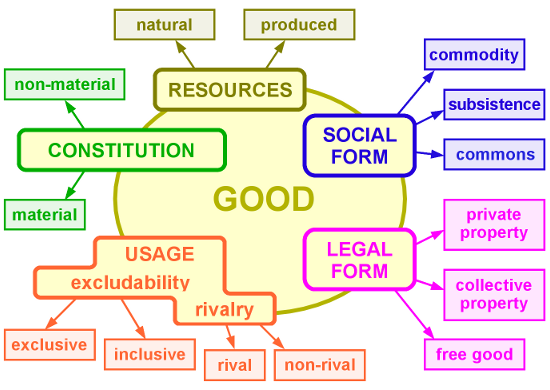
\includegraphics[width=.9\linewidth]{taxonomy-of-goods.png}
	\caption{Taxonomía de bienes o recursos.}
	\todo[inline]{¿Es necesario que el diagrama aparezca en inglés?}
	\label{fig:taxres}
\end{figure}

Volvamos a los factores de producción (tierra, capital y trabajo). El capitalismo necesita disponer de cada uno de ellos de forma que permitan producir más valor para generar más dinero y reproducir el ciclo de acumulación. Ahora bien, para que esto ocurra, necesitamos algo que muchas personas llaman contrato social pero que nosotras preferimos llamar \enquote{reglas del juego}.\revquotes{} Llamemos Estado a la entidad encargada de hacer valer las reglas del juego capitalista a través de las instituciones y de una maquinaria que garantice derechos de propiedad. El Estado proporciona lo que podríamos llamar \emph{aparato de captura} de los factores de producción para el ciclo económico del capitalismo.

Este aparato de captura se compone de tres subjetividades principales: el propietario (que posee la tierra), el banquero (que dispone del capital) y el patrón (que explota el excedente del trabajo). Estas personas (en su mayoría hombres, agentes directos de la estructura social patriarcal del ciudadano) son las cómplices humanas del parásito capitalista y se encargan de perpetuar su existencia garantizando la base material de la producción capitalista. Es decir, son los principales agentes vivos del capital y de su existencia depende estructuralmente la supervivencia del algoritmo. Hemos sido particularmente atentas en explicar estas cuestiones porque entre diferentes posiciones de izquierda (desde marxistas hasta anarquistas, pasando por feministas radicales y ecologistas) resulta extremadamente complicado distinguir al Estado del capitalismo o del mercado, y no podemos pensar en crear una fuerza política que produzca transformaciones radicales sin que entendamos de qué manera se implican estos sujetos en la configuración del estado actual de las cosas.

Hay una dimensión psicosexual de la producción además de sus componentes materiales, a través del deseo. Todas las mercancías son un poco fetiches y actúan como mediadores sociales entre las personas. Las mercancías reflejan lo que las produjo: trabajo y deseo. La relación entre el parásito (capitalismo) y el Estado es simbiótica y no parasitaria. El Imperio es la forma que toma el Estado cuando el parásito muta de la fábrica al algoritmo. El parásito requiere al Estado para garantizar los derechos de propiedad de sus propios agentes.\footnote{(añadir de conspiradores y cómplices).} Estos sujetos son los traficantes de medios de producción y configuran el aparato de captura del Estado (lo que en una configuración urbana serían los muros o en una cárcel las cadenas). La forma algorítmica del parásito, a diferencia de siglos pasados, no reprime ni suprime más el deseo sino que lo recodifica y se deposita en él. Sin embargo, la mutación del capitalismo produce fluctuaciones en el mercado, creando ciclos económicos donde el parásito es más fuerte pero también donde toca fonda antes de volver a mutar.

\begin{figure}[htbp]
	\centering
	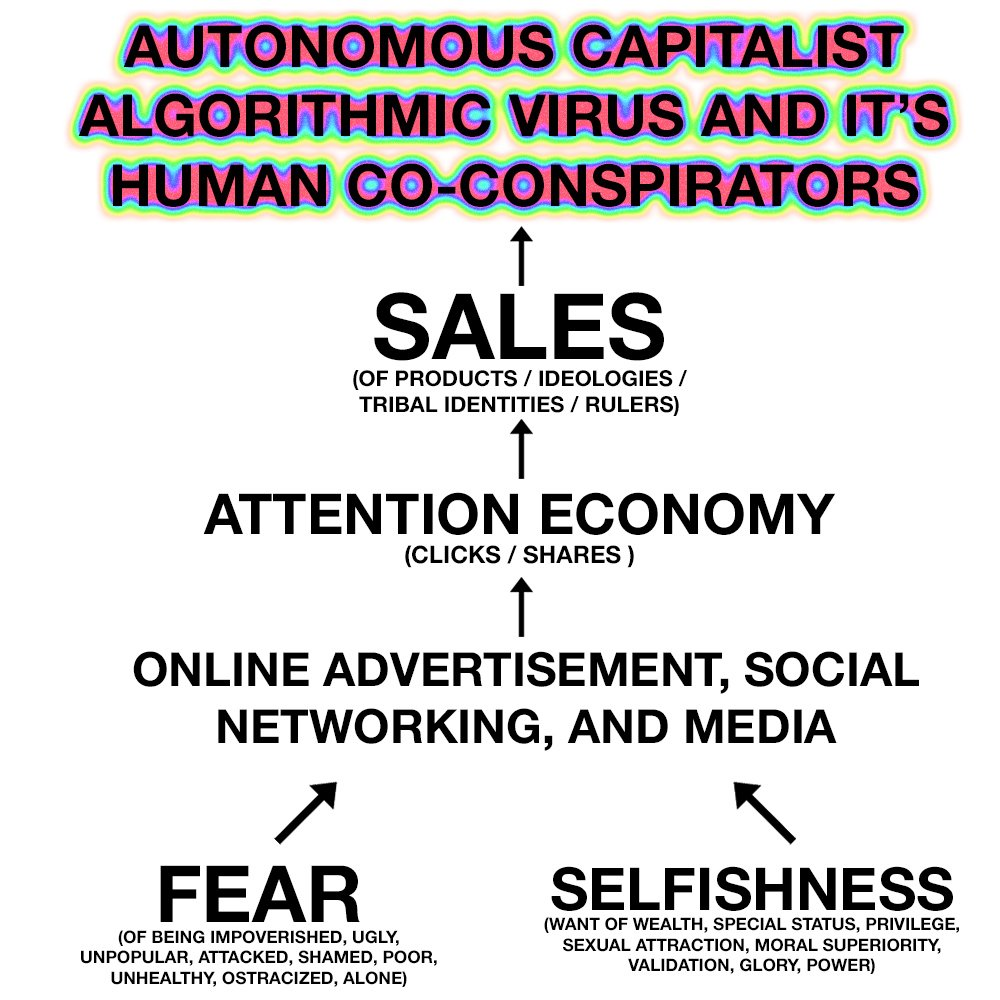
\includegraphics[width=.9\linewidth]{algorithm-capitalism.png}
	\caption[El algoritmo virulento del capitalismo.]{El algoritmo virulento del capitalismo y sus conspiradores humanos.}
	\label{fig:algoritmo}
	\todo[inline]{Valdría la pena rehacer este esquema en español.}
\end{figure}

El parásito infecta a las personas a través de mercancías que producen interacciones sociales a través del intercambio. La persona asalariada, trabajadora, accede a intercambiar su fuerza de trabajo física, intelectual, sexual o la que sea, por la potencia abstracta del dinero y éste por un objeto valorado socialmente que transforma la abstracción del dinero en reputación o prestigio, con el trasfondo del miedo a ser rechazada, a estar fuera del \emph{socius} si una no reproduce la transacción constantemente. De ese modo es que el capitalismo produce subjetividades a partir de la explotación de las trabajadoras, que en realidad no tienen una conexión real con lo que producen. En todo el planeta, aunque a diferentes escalas, esta forma de organización social produce al Gobierno y a sus súbditos: subjetividades caracterizadas por la fórmula \emph{ciudadano soldado consumidor espectador}.

No hay posibilidad de una ciudadanía tal y como se concibe hoy en día al concepto dentro de los Estados liberales democráticos. La subjetividad del ciudadano (soldado, consumidor y espectador) presupone condiciones de clase, etnia y género muy particulares que básicamente se reduce al Señor blanco, heterosexual y cisgénero, que posee propiedades, es patrón de alguien y tiene acceso al crédito y a instrumentos más complejos en el sistema financiero. Además de que esta subjetividad plantea una relación con el cuerpo propio que niega su propia castración,\footnote{Toda mercancía, en la medida en que produce al sujeto como un objeto del valor de cambio de la mercancía, también produce entre sujetos una relación de objetificación. Esta forma alienada, instrumental, de comprender a la otra persona se reproduce en su comprensión de \enquote{lo real}. Es decir, que también produce una idea sobre la naturaleza. De ahí que el capitalismo no produzca otra cosa que hostilidad y desgaste, espacios inhóspitos, pues no concibe al mundo como otro sino como instrumento.} hace creer a la forma de vida que las otras personas son lienzos donde se dibujan sus fantasías frente a otras subjetividades pauperizadas que, entre todas, están construidas para satisfacer los deseos del Señor (¡sí, del Señor feudal, de tu papá y del señor patrón, y del señor de la casa y del Señor que reina en los Cielos, la palabra \emph{Señor} tiene toda esa semántica en tu cabeza!). Entender la realidad de ese modo, y en consecuencia, la Naturaleza (y a Dios, y a la Ciencia, y al progreso), solo reafirma el poder del Estado capitalista. Por ello, cualquier movimiento político que pugne por "corregir al Estado" cuando este es la falla misma, terminará por infectar de deseos señoriales a las formas de vida que resisten a la subordinación del Espíritu que la sociedad moderna produce.\footnote{Aquí, la apuesta del populismo de Ernesto Laclau y Chantal Mouffe se posiciona por la resignificación de estos conceptos en el \enquote{sentido común}.} He ahí la complejidad de la práctica del cambio real.

\section{Más allá del Estado moderno: el Imperio}
\label{sec:imperio}

Desde un punto de vista estratégico, la transformación del Estado moderno tras la consolidación del proyecto imperialista, es el Imperio. Esta forma se caracteriza por una pulverización del poder y un cambio en los modos de producción, donde se privilegian los procesos industriales pulverizados, sin fábricas ni obreros reunidos en un mismo espacio. El Imperio se caracteriza por el auge de entidades más allá de los Estados nación, como las empresas trasnacionales, que compran representantes políticos para legislar en favor de sus intereses. Aunado a lo anterior, la policía y la publicidad, mecanismos del Estado moderno, se transforman en el Biopoder y el Espectáculo.

El Biopoder consiste en el traslado del orden de La Ley a la regulación a través de normas sin sujeto, interiorizadas. Mientras, el Espectáculo consiste en la apropiación capitalista de la imagen para mercantilizar el deseo. Estos procesos maquínicos, que definen al Imperio como fase posterior al desarrollo e implosión de los Estados-nación, tiene distintos modos de regulación, que constituyen y dan forma a su aparato de captura:

\begin{description}
	\item[Aparato socio-ideológico:] familia, tradición, religión, nacionalidad, etc. Codifica el deseo y la colonización psicológica del sujeto, establece hegemonía además de producir y mantener el estado actual de las cosas.

	\item[Aparato productivo-comercial:] finanzas, bancos, empresas corporativas, propietarios, etc. Comercialización de la producción, mercantilización del deseo para ligarlo al proceso de producción, monopolización del mercado, el valor de los desvíos que vuelve a los ricos a través de la parasitación de la mano de obra.

	\item[Aparato marcial-carcelario:] los militares, la policía, la inteligencia, el sistema de prisiones. Mantiene el estado actual de las cosas a la fuerza, la disciplina y el control de los sujetos, protege los intereses de los propietarios capitalistas y del Estado, sus fronteras, extrae recursos de otras regiones a través de la fuerza, redirige la riqueza para expandir el brazo militar del Estado e incentiva su investigación y desarrollo.

	\item[Aparato subversivo-periférico:] subjetividades colonizadas, grupos minoritarios, organizaciones criminales, la banda en sombra (\emph{shadow banking}), los mercados negros, etc. Muerte social y necropolítica. Establece la identidad de los ciudadanos mediante la otredad como diferenciación de subjetividades marginales, da un camino al lucro más allá del aparato comercial productivo.

	\item[Aparato legal de la soberanía:] el Estado, el sistema de justicia, los gobiernos, etc. Colonización el espacio geofísico, establecimiento del territorio y determinación de estratos y jerarquías sociales.
\end{description}

\begin{figure}[htbp]
	\centering
	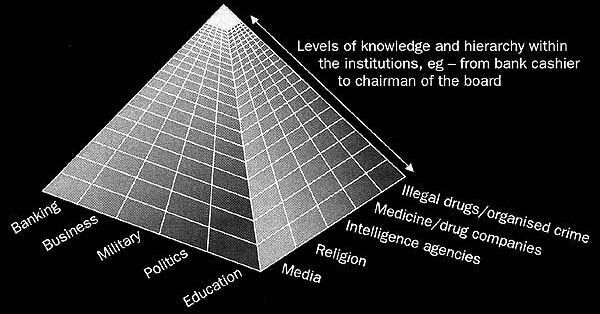
\includegraphics[width=.9\linewidth]{hierarchy-piramid.png}
	\caption{Taxonomía de bienes o recursos.}
	\label{fig:piramide}
\end{figure}

Si le damos una pensada más profunda y concreta, descubriremos que detrás de cada uno de estos dispositivos existen entidades económicas con transacciones y reglas del juego que regulan la vida social en diferentes esferas pero a dos escalas, una micro (corporal, que corresponde al Biopoder y el Espectáculo) y macro (burocrática, de legislación e infraestructura tecnológica). En principio, podríamos hablar de las cinco grandes empresas que condicionan el desarrollo de las telecomunicaciones: Amazon, Apple, Google, Microsoft y Facebook. Estas son la base material por donde fluyen información y códigos sociales, representaciones del mundo, que son reproducidas en los dispositivos personales para provocar una reacción, un deseo. Esta nueva forma del capital explota reacciones, capitaliza el placer que puede cuantificar en \emph{clicks} y \emph{shares}.

Este ciclo se basa en un delicado circuito de excitación, frustración y excitación que regula los hábitos de consumo. Se trata del modelo ideal de empresa neoliberal, un paradigma del negocio pos-industrial. La pornografía es un régimen estético que produce significados y un modo de presentación de las cosas que resulta adictivo, que permite obtener satisfacción del placer masturbatorio sobre la representación de cualquier fantasía posible materializada en videos.\footnote{De cierto modo, que el capitalismo se presente actualmente en su mayor apogeo a través de la industria farmacopornográfica (régimen toxicológico y semiótico-técnico), reproduce una concepción de la subjetividad como no castrable, cuyo horizonte parece ser el de autómatas dependientes del \emph{soma} de Huxley, personas discapacitadas, incapaces de habitar, de subsistir autónomamente.} En los foros de internet para varones adictos a la pornografía existe un nombre para el circuito pornográfico que tiene atados a tantos hombres a una forma particular de desear. Se conoce como: \emph{Porn, Masturbation, Orgasm (PMO)}.\footnote{Reddit. \emph{Don't lie to yourself\ldots P-M-O (PORN\ldots masturbation and orgasm) IS THE PROBLEM. Masturbation is just the symptom.} Disponible en \url{bit.ly/2HuEoem}.} El malestar de estos hombres cada vez más incapaces de vivir y en simbiosis con las comodidades del capitalismo que extienden el poder de sus formas tristes de vivir a otras esferas sociales, son el síntoma de este nuevo rostro de la economía. La excitación, la erección, la eyaculación, el placer y el sentimiento de autocomplacencia y control omnipotente se vuelven materias primas del proceso productivo.

\begin{figure}[htbp]
	\centering
	
\includegraphics[width=.9\linewidth]{nofap.png}
	\caption[Movimiento noFap.]{Movimiento noFap para hombres adictos a la pornografía y a la masturbación.}
	\label{fig:noFap}
\end{figure}

Por esta razón, P. Preciado señala que la pornografía es el rostro desenmascarado de la industria de la cultura y propone el concepto de \emph{farmacopornografía} para referirse al gobierno biomolecular y semiótico-técnico de la subjetividad sexual. Hay, de hecho, empresas que se encargan de regular la producción de contenidos excitantes que funcionan como mercancías con estudios explotadores y personas trabajadoras sexuales explotadas. La explotación mercantil del sexo es paradigmática porque un solo video puede producir millones de orgasmos,\footnote{Vale la pena revisar las estadísticas del tráfico de pornografía en internet. Por ejemplo, la información que libera \href{www.pornhub.com/insights/category/stats}{PornHub}.} lo que contrasta con la industria farmacéutica, donde el desarrollo de un medicamento cuesta muchísimo pero es fácilmente reproducible una vez que se obtiene y patenta una fórmula.

\begin{figure}[htbp]
	\centering
	
\includegraphics[width=\linewidth]{pillAd1.png}
	\caption{Anuncio de la píldora anticonceptiva.}
	\label{fig:anticonceptiva}
\end{figure}

\begin{figure}[htbp]
	\centering
	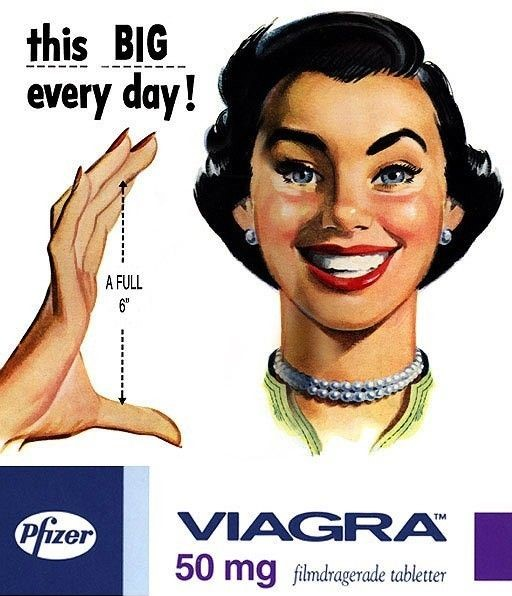
\includegraphics[width=\linewidth]{pillAd2.jpg}
	\caption{Anuncio del viagra.}
	\label{fig:viagra}
\end{figure}

Así, las grandes entidades económicas capitalizan problemas clásicos de la economía como las asimetrías de información, el problema de agencia o los dilemas de acción colectiva. Además, condicionan nuestros deseos imprimiendo en nuestras psiques imágenes de lo deseable, además de crear una erística que nos enseña que esos estímulos que aprendemos a desear los podemos obtener a través de la moneda, de intercambios mercantiles. Estas empresas aprenden a través de costosas investigaciones sobre el comportamiento humano, para reproducir la servidumbre en los contenidos a través de segmentos de mercado donde se puede insertar el discurso del parásito capitalista bajo distintas situaciones y formas sexuales. PornHub es el paradigma de la industria cultural por su capacidad para producir orgasmos, para \emph{gestionar el género, la excitación, la frustración y el placer}. De este modelo de empresa se pueden extender otras versiones \emph{soft} (o blandas) que operan en otros aparatos sociales. Disney como el dispositivo que reproduce el imaginario de la jerarquía social a través de sus mitos de princesas, reyes y monstruos; MacDonalds y Coca Cola para reproducir la \hlfix{chatarrofagia}{Resaltar en cursivas.}.\footnote{Es decir, la enfermedad de la impotencia, del cuerpo enfermo, pauperizado, envenenado por las bombas mediáticas que producen la comida rápida o chatarra como lo deseable, como el lugar a donde gastar el salario. Se trata de un régimen alimenticio de productos vacíos, compuestos de harinas, grasas, azúcares y otras sustancias que funcionan bajo el mismo principio de estimulación-malestar y que producen serios daños al cuerpo a largo plazo. El paradigma mercantil de la comida en tiempos del Imperio.}

\begin{figure}[htbp]
	\centering
	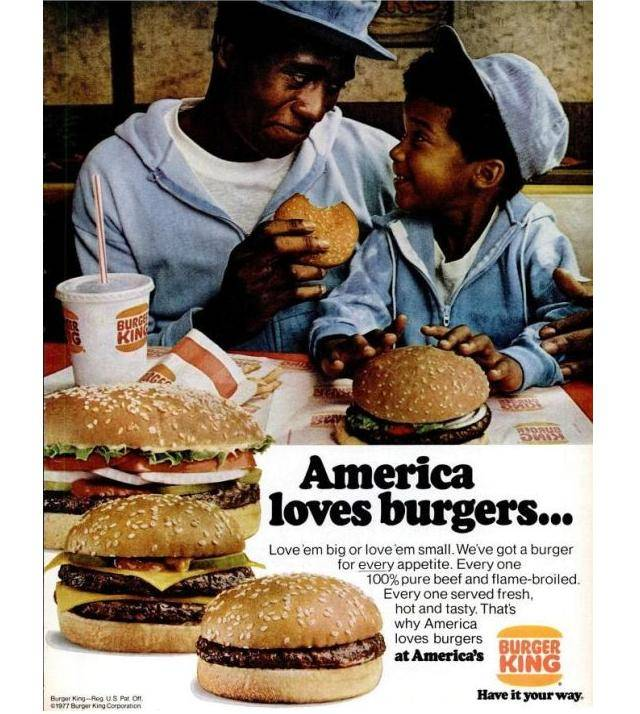
\includegraphics[width=\linewidth]{burguers.jpg}
	\caption{¡América ama las hamburguesas!.}
	\label{fig:burger}
\end{figure}

\section{La vida como trabajo y la producción de subjetividad}
\label{sec:subjetividad}

Un punto importante para comprender la transformación del Estado-nación al Imperio se encuentra en el papel del trabajo. Por ello, en este apartado analizaremos las condiciones de producción del trabajo del hombre-masa en la era cibernética. Para comenzar, tenemos que recordar que la dominación mercantil tiende a expandir sus dominios a toda área de la vida y al hacerlo vuelve trabajo a cualquier acción sujeta de la explotación. Este proceso está relacionado con la transformación de la subjetividad. No por nada el concepto central de las revoluciones de los siglos XIX y XX es la masa, una subjetividad que experimenta la realidad de la misma manera, a través del \emph{consumo estandarizado}. En este proceso, las vivencias en su forma de experiencias cognitivas dan sentido y estructura a la imaginación, es decir a la máquina deseante que es cada singularidad. Así se configura una idea del pasado (a través de Hollywood que nos enseña a desear melancólica o espectacularmente) y del futuro (el apocalipsis como una finalidad de la historia implícita en las narrativas culturales a través del tecnocapitalismo, donde la explotación se extiende a cada rincón del planeta, deja a su paso desolación y muerte para después reconstruir la \enquote{sociedad}\revquotes{}) a través de los medios que producen para las grandes audiencias.\footnote{Que dan forma a la cultura popular y al espectador televisivo en un circuito que lo posiciona como ente pasivo sentado en un sillón consumiendo comida chatarra.}

En términos concretos, la masa es el resultado de un proceso sintético en el que el individuo afronta una situación externa a él, participa en la situación y proyecta la situación en otros individuos que habitan el mismo espacio. Como ejemplo está Disney, que transmite efectivamente el deseo de casta a través de sus figuras de princesas, reyes y caballeros. Para profundizar sobre estos puntos conviene revisar los documentales de Adam Curtis, particularmente recomendamos \emph{The Century of the Self} y \emph{Hypernormalisation}.

\begin{figure}[htbp]
	\centering
	
\includegraphics[width=.9\linewidth]{complicated.jpg}
	\caption[\emph{Hypernormalisation}]{Toma de \emph{Hypernormalisation}.}
	\label{fig:hypernormalisation}
\end{figure}

Nosotras hemos intentado perfilar a la subjetividad ideal del Estado moderno como algo parecido al \emph{ciudadano soldado consumidor espectador.} Solo basta recordar que el antecedente histórico del ciudadano han sido los súbditos, los fieles. Quizá desde ahí se perfila el proceso donde las multitudes devienen siempre masa a través de los aparatos de captura. El lenguaje cotidiano es muy útil para hacernos ver cómo se transmite la deuda en la subjetividad de ciudadano soldado consumidor espectador:

\begin{quote}
	paga tus impuestos\\ 
	sirve a la patria\\
	no te pierdas el descuento\ldots{}\\ 
	ni el siguiente show (la siguiente película).
\end{quote}

En esta fórmula todas las personas deben. El deber y la deuda provienen del mismo sentir (y de la misma locución latina \emph{debere}). Sin embargo, la deuda tiene una condición que ha sido entregada antes del nacimiento, como una suerte de fruto por el que hay que pagar con el pecado original durante el resto de nuestras vidas. El ciudadano \emph{debe} pagar sus impuestos, el soldado \emph{debe} honrar a la Patria, el consumidor \emph{debe} comprar y el espectador \emph{debe} mirar.

\section{Hoy en día, el capitalismo se comporta como un virus}
\label{sec:viruscapitalista}

El algoritmo del virus capitalista y el condicionamiento de desarrollo de las tecnologías mediáticas para el excedente configuran lo que se espera de las personas individualmente a gran escala. Si bien los Estados-nación dieron forma a las revoluciones burguesas fue en parte por la capacidad de leer la prensa escrita como criterio de consumo literario común suficiente para dar forma a una identidad colectiva, a una identidad de clase. Después, la radio y el cine también configuraron el potencial revolucionario de las comunicaciones. Por ejemplo, el radio creó un espacio informacional nuevo (urbanismo y psicogeografía). Esto nos muestra cómo una forma mediática representa poder y nos revela el papel clave de los \emph{medios}. Lo hace configurando el espacio a través de flujos de comunicación. La configuración de estas redes de comunicación es un catalizador para el cambio social (tabla~\ref{tab:Aristas} página~\pageref{tab:Aristas}).

En la actualidad, los modelos de masa donde un grupo recibe una sola transmisión son reemplazados por modelos donde el individuo recibe una transmisión única gracias a algoritmos reactivos que alteran la secuencia del contenido de las redes sociales y de ese modo individualiza y hace única la experiencia de consumo de cultura. La subjetividad ya no es producida como individuos en serie sino a través de segmentos.

El cambio de paradigma de modelos de gobernanza en masa a modelos en red obedece al desarrollo cibernético del algoritmo. Las sociedades disciplinarias y de control son demasiado complejas para gestionar, por lo que es más fácil fijar protocolos para gestionar redes de manera más eficiente. El espacio masivo está condicionado al número de participantes en un espacio y un momento particulares mientras que el espacio de redes se extiende y contrae en el espacio-tiempo de acuerdo a las órdenes y necesidades de la red. Es decir, su uso del capital es más eficiente porque se ajusta a las necesidades de cada momento.

Hasta ahora, este capítulo ha sido fuertemente influenciado por textos apócrifos de \#altwoke. Una idea discutida por la wikiPartida (una instancia de la Partida compuesta por gente de Wikipolítica) a partir de lo expuesto es que los modelos de gobernanza en red pueden desarrollar y expandir una cultura a través de \emph{labels}, donde los participantes son suscriptores de esta. Esto para hacer frente al problema de cómo se desplegaría una identidad FLOS que transmita cierta disposición práctica en los logos de organizaciones que la adopten. Por otro lado, nos surgen preguntas referentes a la cuestión de los medios como:

\begin{itemize}
	\item ¿qué ocurre con los gobiernos coloniales con el consumo de medios si hay masas y segmentos conviviendo y entrecruzándose? Nos referimos a medios como Netflix, Spotify y plataformas en línea además de Disney, DirecTv, Warner o, en el caso de México, Televisa.
	\item ¿Cómo se configura el imaginario de las personas en México entre Facebook, Twitter, Instagram o YouTube por un lado y Televisa, como el monopolio de sentido durante el siglo XX por el otro? Sin mencionar a Bimbo, Walmart, Coca Cola y otros grandes leviatanes. 
\end{itemize}

\section{Alternativas económicas para el futuro}
\label{sec:altfutur}

\begin{figure}[htbp]
	\centering
	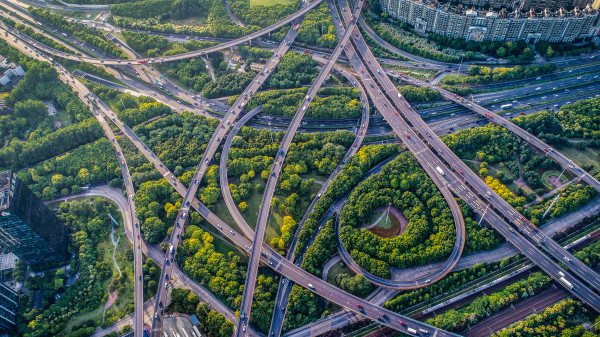
\includegraphics[width=.9\linewidth]{roads.jpg}
	\caption[\emph{Hypernormalisation}]{Toma de \emph{Hypernormalisation}.}
	\label{fig:hypernormalisation2}
\end{figure}

Hemos visto que en el entramado de complejas tecnologías que dan forma al presente, resulta extremadamente difícil accionar sin reproducir la lógica de la sociedad mercantil. El Estado, los mercados y el capital producen en conjunto una sociedad unida por un acuerdo económico donde la ética tiene un papel tan nulo que debe ser enunciada a través de imperativos morales universales porque nadie cree en ella. Y esto porque la sociedad es, en realidad, un arreglo para dar vida a las mercancías. No hay nada vivo ahí. Tiqqun acertó en señalar que la antítesis del comunismo no es el capitalismo sino la economía, y que lo que es necesario derrumbar es la dominación mercantil, que se asume como realidad última de todas las formas de vida y de todas las cosas. Para concebir acciones efectivas y críticas, tenemos que considerar que nuestras prácticas deben rebasar las estructuras formales e informales que reproducen al parásito capitalista. Para ello es de gran utilidad asumir una visión interseccional centrada en la \emph{interacción entre violencias estructurales (género, raza\footnote{Hemos utilizado la palabra raza para referirnos al discurso de raza, una ideología biologicista que sirve a los patriarcas blancos para justificar la opresión a grupos étnicos o a cualquier forma de vida no-blanca.} y clase), dispositivos sociales, el aparato de captura del Estado, la cadena de producción del capitalismo contemporáneo y el algoritmo del virus capitalista}. Esto en un contexto de complejidad donde la producción económica es comprendida en buena medida como informática, como flujos de datos con potencial de explotación. La visión de la economía neoclásica, que al informatizar la economía, le da forma de cibernética, también puede ser una herramienta de sabotaje si pensamos en los problemas de acción colectiva que necesitamos resolver para combatir la dominación mercantil como problemas de información. Algunos ejemplos que pueden ser analizados bajo esta óptica son:

\begin{description}
	\item[Gobierno representativo:] entender a los representantes como traficantes de información sobre los incentivos de sus representados (lo que en economía se conoce como \enquote{problema de agencia}\revquotes{} o \enquote{problema de agente-principal}\revquotes{}).

	\item[Burocracia:] cualquier burócrata sabe que una parte importante de la función del gobierno es el procesamiento de certificados y documentos. Una alternativa es pensar que la burocracia sea reemplazada por programadoras que mantengan un modelo de gobernanza como una máquina de información en FLOS.

	\item[Cambio climático:] un sistema de gobernanza efectivo tiene que permitirnos reconocer los costos reales y las externalidades de la producción para administrarlas en un equilibrio de Pareto.
\end{description}

Además de eso, tenemos que plantear una lógica económica para producir redes de economía solidaria que a su vez produzcan otras economías del deseo. Es decir, tenemos que combatir desde el aspecto de la infraestructura y superestructura que dan vida a la sociedad, mientras que generamos otras plataformas para producciones autónomas de deseo. Tanto la lucha por un nuevo poder constituyente como la de prácticas de destitución del Estado capitalista encuentran un entrecruzamiento en las tecnologías que condicionan su desarrollo. En ese sentido, la disciplina que se ocupa por comprender, visibilizar y transformar las relaciones de poder y sus condiciones de posibilidad[\textsuperscript{20}] en este momento histórico bien puede ser nombrada \emph{tecnocrítica}.

\begin{figure}[htbp]
	\centering
	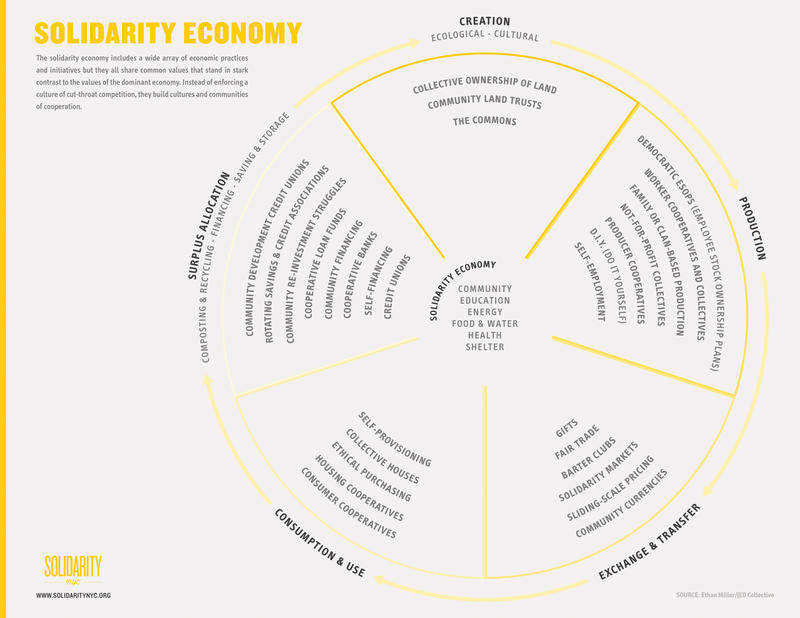
\includegraphics[width=.9\linewidth]{solidarity-economy.jpg}
	\caption{Economía solidaria.}
	\label{fig:solidarieco}
\end{figure}

Una economía tecnocrítica debería basarse en cadenas de producción que sean cíclicas y ecológicas, además de proponer trabajos orientados a la economía de la regeneración para generar empleos que restauren el medio ambiente.

\begin{figure}[htbp]
	\centering
	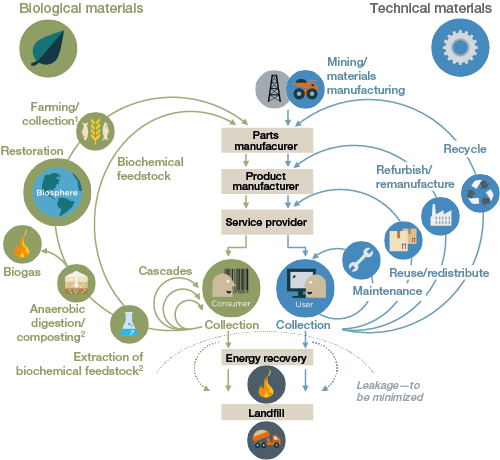
\includegraphics[width=.9\linewidth]{circular-economy.png}
	\caption{Economía circular.}
	\label{fig:circuleco}
\end{figure}

Frente a la falta de fundamentos teóricos de muchas propuestas políticas contemporáneas, nosotras creemos que el mundo donde caben muchos mundos se nutre de \emph{una ecosofía (un saber desde la Tierra), xenofeminista (que entiende las formas de opresión como el género, la raza o la clase social como tecnologías) e interseccional (que considera que distintas violencias se intersectan en las subjetividades)}. Es a partir de esta posición que tiene sentido para nosotras pensar una consideración estratégica sobre la práctica política. Hay que ir más allá de las adherencias identitarias a una facción política. Por ejemplo, la dialéctica entre horizontalismo y verticalidad es un falso dilema, ambas formas conviven en todas las relaciones grupales. Más allá de una nomenclatura en particular, nuestra posición siempre es tecnopolítica y busca prácticas anticapitalistas y antiestatales, creando comunes que permitan la gobernanza de grupos que pueden reapropiarse el valor del globalismo, descentralización, sociocracia, etc, entendiendo las subjetividades más allá del control administrativo central de la sociedad, es decir, de las normas que configuran los vínculos sociales.

La economía del don es parte de la visión de los comunes. Existen ejemplos como Grameen Bank que contribuyeron a terminar con la situación de pobreza de muchas personas en la India. Pese a que reproduce en cierto grado la lógica que las produce, sí logran generar un cambio de alto impacto. Es decir, escalable. Se trata de hacer modelos para descubrir, por ejemplo, cuántas vidas puede salvar tu proyecto, qué tan capaz es de visibilizar y crear alternativas a las violencias estructurales que sufre una persona, y encontrar proyectos clave que reduzcan transversalmente distintas formas de violencia al mismo tiempo, algo parecido al principio de Pareto.

El punto central de este apartado es señalar que la imaginación política presupone ciertas formas de hackeo a los dispositivos que dan fuerza a todo el embrujo mercantil, que son las formas abstractas de valor. El arte y el dinero tienen una relación importante en cuya génesis se pueden explorar algunas posibilidades de emancipación. La meta es reducir la dominación mercantil en estructuras económicas productivas.

\begin{figure}[htbp]
	\centering
	
\includegraphics[width=0.6	\linewidth]{artAfterMoney.jpg}
	\caption[Recomendamos el texto de Max Haiven.]{Recomendamos el texto de nuestro colega Max Haiven.}
	\label{fig:Haiven}
\end{figure}
\chapter{Principios para la acción efectiva}
\label{cha:principios}

Por ahora, frente a la acelerada decadencia de nuestros vínculos políticos, creemos que es necesario crear un ecosistema de tecnologías cívicas para hacer efectivas las garantías jurídicas a las personas ciudadanas que, por sus condiciones particulares, no pueden tener acceso a la justicia o al gobierno. Este movimiento tiene que luchar por una cultura pirata, es decir, concentrada en hacer libres, abiertos y accesibles todos los recursos de los que dispone. De la misma manera, necesitamos desarrollar principios de política pública, de economía y de gobierno, que se vuelvan el sentido común de tanto de las planificadoras como de las estudiantes de las escuelas de negocios y de administración. En cierto sentido, se trata de desarrollar un nuevo pensamiento económico que haga frente a la visión neoclásica de entidades racionales y maximizadoras de utilidades. En cuanto a nuestra estrategia, nos reconocemos en una tensión entre la transparencia y la opacidad.\todo{Desarrollar.} Sabemos que el humor juega un papel fundamental en la conformación de un nuevo imaginario político. Hasta ahora, hemos pensado en algunos principios como parte de una visión efectiva de la táctica política progresista:

\section{Pragmatismo no es utilitarismo}
\label{sec:pragmatismo}

Muchas personas casadas con la Teoría crítica (marxismos, psicoanálisis, etcétera) satanizan la filosofía del hacer efectivo y eficiente. Nosotras pensamos que esta actitud de repudio a la estadística, a la optimización y a la eficacia son lo que nos ha valido tantas derrotas. Podemos pensar las cosas más románticas del mundo sobre la revolución, pero la realidad es que toda operación requiere un pensamiento estratégico, requiere instancias (es decir, medios concretos de ejecución, como el código en computación) y que no lograremos disputarle el sentido común al neoliberalismo, ni imaginar un más allá del Estado o del capitalismo si no pensamos que teoría, estrategia y práctica están interrelacionados y que no bastan buenas intenciones. Como lo señala Alinsky en su Tratado para radicales, las cuestiones morales no tienen ningún sentido frente a nuestros enemigos. Ahí mismo señala que la historia nos ha enseñado que primero se toma la acción y después se legitima.

\begin{figure}[htbp]
	\centering
	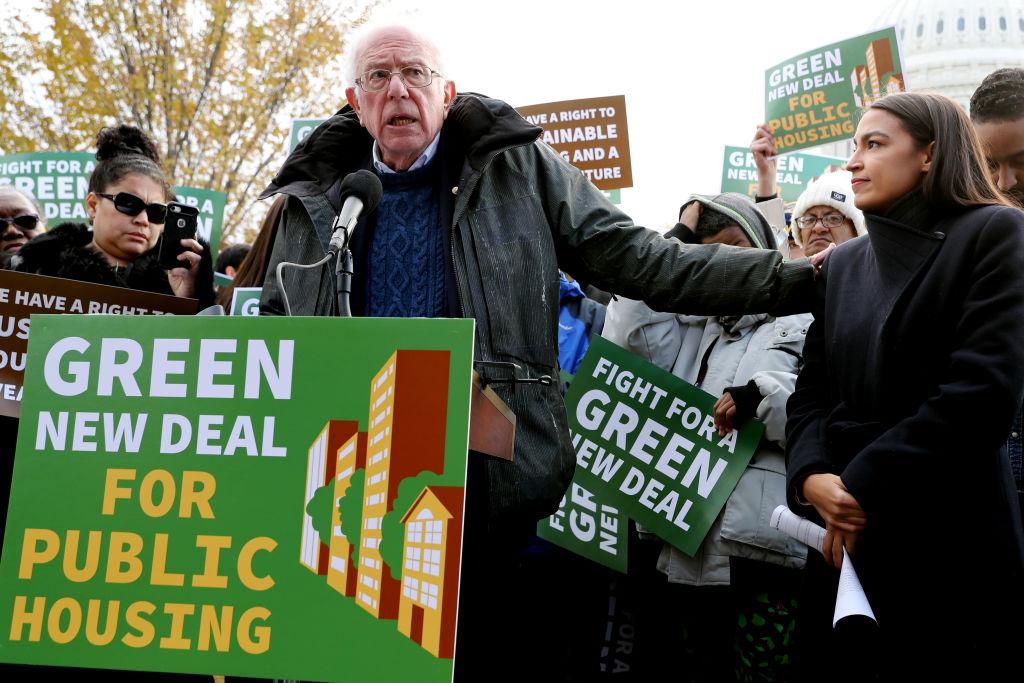
\includegraphics[width=0.8\linewidth]{green.jpg}
	\caption[Buen ejemplo de pragmatismo con sentido.]{Bernie Sanders, Alexandria Ocasio Cortés y el \emph{Green New Deal} son un buen ejemplo de pragmatismo con sentido.}
\end{figure}

\section{Interseccionalidad en la acción}
\label{sec:interseccionalidad}

Que todas nuestras acciones estén centradas en atender las condiciones estructurales de opresión a través de un movimiento emancipatorio que busque hacer frente de forma transversal a las diversas formas de violencia que padecen las personas. Para lograrlo, es necesario que entendamos cómo funciona el capitalismo hoy en día, en un contexto donde la fuerza de trabajo está totalmente precarizada, pulverizada y disuelta, en una época económica conocida como posfordismo, que consiste en una era donde la producción está profundamente ligada a la teoría de la información y de la computación. La interseccionalidad nos obliga a concentrarnos en desarrollar herramientas para comprender cómo funciona la explotación en sus distintas formas, por ejemplo, cómo se intersectan las violencias de género, racistas y de clase.

\begin{figure}[htbp]
	\centering
	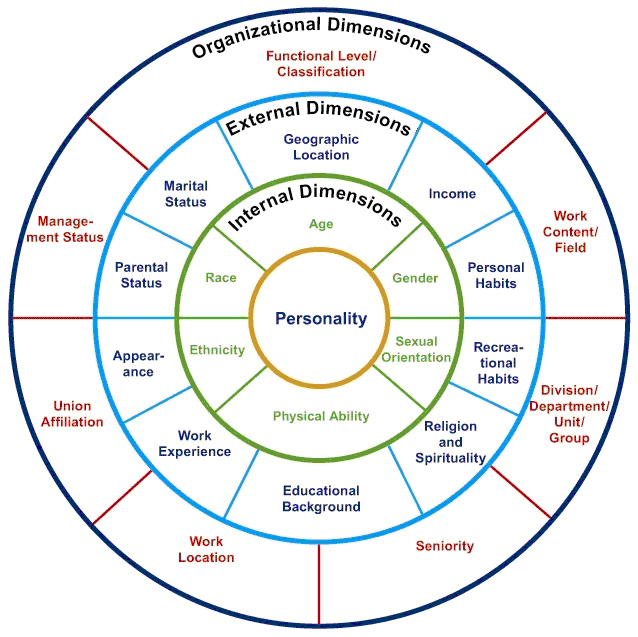
\includegraphics[width=\linewidth]{self-dimensions.png}
	\caption[Dimensiones de la personalidad.]{Dimensiones de la personalidad y factores de influencia.}
	\label{fig:dimensiones}
\end{figure}

\section{Transmisibilidad, o sea, hacernos accesibles}
\label{sec:transmisibilidad}

Si la ideología es el conjunto de significados culturales que nos hacen estar a favor o en contra de algo, necesitamos crear mecanismos de reconocimiento y traducción de estos significados para poder transformarlos. La mayoría de las personas no está realmente convencida de todo lo que cree y muchas veces lo cree más por ser receptora de un flujo de imágenes o de opiniones de gente con reputación social, que por su propio convencimiento. Ese es nuestro objetivo, ser capaces de comunicar a esas personas una visión comprensiva de la diferencia, de la otredad, de la dignidad del prójimo. Debemos hacer que nuestro discurso sea trans-ideológico, que pueda dialogar con distintas visiones reapropiándose y resignificando conceptos cooptados por conservadores y tradicionalistas (es decir, la derecha). Esta idea es parecida a lo que en ciencias sociales se conoce como intersubjetividad, que es la capacidad de las hablantes de crear significados comunes y compartidos que configuran su sentido común. Para lograr ser transmisibles, necesitamos más mercadotecnia para transmitir una cultura crítica y para comunicar el feminismo y la teoría crítica a gente que sabemos que podría accionar hacia una causa en particular, induciendo una disonancia cognitiva.\todo{Definiri disonancia cognitiva.} Pensémoslo como si estas personas fueran \emph{swing voters} que tienen que elegir entre el sentido común neoliberal que las aliena o una visión crítica que las ayuda a reconocerse como personas con dignidad más allá de los códigos sociales. Pero no podemos hacer esto si no pensamos en los códigos de quienes nos escuchan. En el Corán, la \emph{taqiyya} o \emph{kitman} es el acto de disimular nuestras propias creencias en tiempos de persecución. Necesitamos disimular nuestras creencias y visibilizar mensajes seleccionado cuidadosamente para que logren insertarse en los flujos de deseo del capitalismo sin que el enemigo nos reconozca.

\begin{figure}[htbp]
	\centering
	
\includegraphics[width=\linewidth]{he4she.jpg}
	\caption[Emma Watson, vocera del \emph{He for She}.]{Emma Watson, vocera del \emph{He for She}, una forma de \emph{mainstreaming}.}
	\label{fig:he4she}
\end{figure}

\section{FLOS y la bandera pirata}
\label{sec:FLOS}

En la jerga \hlfix{geek}{En cursivas.}, \emph{Free/Libre and Open Source Software} (FLOSS) es el tipo de software accesible a través de su código fuente. Esta filosofía es absolutamente necesaria para una práctica que permita el autogobierno de las personas y reduzca la dependencia al Estado y a los mecanismos tradicionales de gobierno, así como el poder de mercado de las corporaciones a través de las patentes. Nosotras añadiríamos \emph{Free/Libre and Open Source Culture} (FLOSC) para referirnos a un desarrollo en la cultura donde los procesos de creación de valor y de desarrollo de productos sean visibles y no ideológicos, es decir, que sirvan para que más gente pueda producir sus propios significados y sus propias estéticas y no para que sea utilizado para que la gente reproduzca un modelo de consumo (que es la función de la ideología). La cultura FLOS debe extenderse al espacio público, a la Academia, a los mercados (que hoy en día pertenecen a horribles lagartos que, a través de cinco empresas, controlan los flujos de distribución de mercancías y de imágenes en todo el planeta), a la educación y a todas las instituciones que reproducen el estado actual de las cosas. Esto significaría que el gobierno deje de operar empresas estatales y que más bien permita sus operaciones públicas, a través de certificaciones y procesos de descentralización, y no a través de la concesión a grandes monopolios transnacionales.\footnote{Entendemos, sin embargo, que hay problemas importantes cuando pensamos en proyectos que son intensivos en capital, como grandes obras de infraestructura o complejas investigaciones médicas. También se trata de acelerar los procesos de democratización y de FLOS dentro de la estructura de las corporaciones, que hoy en día, son reinos con el todopoderoso CEO (\emph{Chief Executive Officer} o director general) gobierna sobre todos sus súbditos a través del salario.}

Respecto a la cuestión de las patentes, hay ideas muy interesantes como el \emph{copyleft} o el \emph{copyfair} que buscan reformular patentes y crear esquemas que fomenten cooperativas. Nosotras pensamos que este tipo de prácticas podrían servir en las licitaciones gubernamentales para generar leyes que obliguen a las instituciones públicas a tener procesos y patrones de cultura FLOS.

Otra idea con la que hemos coqueteado es con las etiquetas o \emph{labels} en inglés. Por ejemplo, una etiqueta \emph{Low tech} que certifique que ciertos productos desarrollados fueron diseñados como alternativas a la obsolescencia programada y con la posibilidad de intervenir sobre ellos. La idea de la etiqueta surge como una forma de crear un sistema de certificados que pueda competir con la lógica capitalista de producción de las grandes marcas, con la intención de desacelerar los ciclos de producción y consumo.

Algunas referencias interesantes para complementar este apartado:

\url{http://unenumerated.blogspot.com/2017/02/money-blockchains-and-social-scalability.html}

\url{http://unenumerated.blogspot.com/2006/11/wet-code-and-dry.html}

\begin{figure}[htbp]
	\centering
	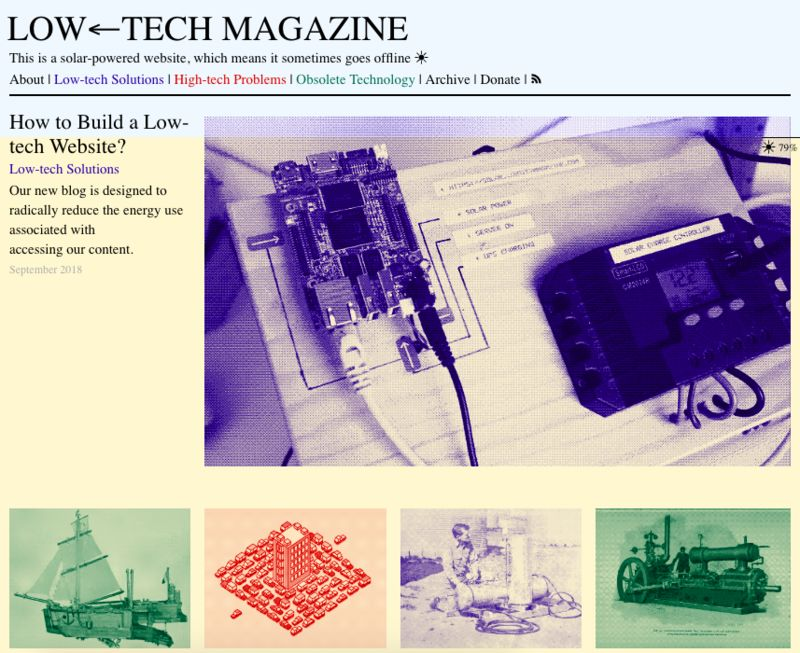
\includegraphics[width=.9\linewidth]{low-tech.jpeg}
	\caption[\emph{Low Tech Magazine}]{Imagen del sitio \emph{Low Tech Magazine}.}
	\label{fig:lowtech}
\end{figure}

\section{Queremos un mundo más allá de la economía capitalista}
\label{sec:mundo}

Algunas personas dicen que incluso si acabáramos con el capitalismo como forma de explotación, todavía habría que pensar en cómo ir más allá de relaciones sociales mediadas por abstracciones como la moneda. ¿Por qué? Cada vez presenciamos cómo hasta la última esfera de la vida está sujeta a la regulación, a la medición y a la cuantificación. Esto nos impide vivir sin considerarnos a través de márgenes de utilidad y hace que nos sigamos mirando las unas a las otras, al menos parcialmente, como objetos de interés. La cibernética es la ciencia y arte del control que cuantifica cada vez más toda experiencia de vivir en \emph{clicks}, en \emph{shares}, en \emph{likes}, y esto no hace sino aumentar el deseo de enjuiciarnos cada vez más. Una posible solución está en pensar que las tecnologías que desarrollemos para crear un Estado más justo también tienen que preguntarse cómo haremos para generar más vínculos, más encuentros donde las personas puedan hablar, escucharse y establecer vínculos más allá de la pertenencia a una tribu identitaria o a cualquier grupo de interés. Creemos que el verdadero problema de la tecnología es su desarrollo capitalista, que desorganiza a las personas para volverse cada vez más necesaria.

Para lograrlo, podemos valernos de investigaciones como \emph{Nudge economy}, parte de la economía de la conducta que analiza el diseño de incentivos que conducen a la gente a tomar decisiones, es decir, la disposición económica de los objetos a las personas. En este campo es también posible vincular la experiencia de usuario o UX (\emph{user experience}) para hacer interfaces más accesibles e incluso más comunitarias.

\begin{figure}[htbp]
	\centering
	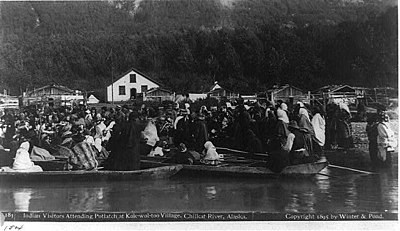
\includegraphics[width=\linewidth]{potlatch.jpg}
	\caption[\emph{Potlatch}.]{El \emph{potlatch}, concepto clave en la economía del don de Marcell Mauss, es un ritual de los pueblos aborígenes de la costa del Pacífico en el noroeste de Norteamérica, tanto en los Estados Unidos como en la provincia de la Columbia Británica de Canadá. EE.UU.}
	\todo[inline]{Corregir el brillo y contraste de la imagen para que se pueda ver con más claridad.}
	\label{fig:potlatch}
\end{figure}

\section{Luchemos por estar en los canales masivos}
\label{sec:luchemos}

El algoritmo del capitalismo funciona implantándonos deseos de consumir y de cumplir ciertos códigos sociales que siempre tienden al individualismo y a la mercantilización de las otras personas. No creemos en la falsa dicotomía entre luchas locales y globales, creemos que hoy en día, toda forma de activismo es una cierta tecnopolítica. Es decir, que nuestras prácticas contienen cierta posición estratégica sobre el uso de los recursos en decisiones tan básicas como usar manuales de \emph{zero waste} en eventos públicos y hacer campañas para hacerlo una moda. Si realmente queremos hacer algo efectivo, tenemos que crear un \emph{mainstream} o corriente mayoritaria que permita unir distintos proyectos que luchan por la emancipación así como los ingleses tienen BBC como distintivo de su identidad y de su cultura.

El trueque, el \emph{freeganism} o los bancos de tiempo son estrategias de resistencia que por sí solas, aisladas en contextos locales, de micropolítica, no pueden hacer nada para ganarle a los millones de dólares que la industria de la comida rápida invierte en hacernos desear el azúcar, las grasas y cualquiera de esas sustancias que nos restan salud. Sin embargo, combinadas en una campaña masiva y consolidando audiencias que puedan encontrar alternativas sistémicas como salud pública y comedores comunitarios, empezaremos a tener victorias reales. Es decir, hay que crear flujos alternativos a la cultura de masas que tengan aspiren a una plataforma común de organización, para hacer publicidad no a un proyecto de bajo impacto en particular, sino a una alternativa sistémica y escalable. Para nosotras, Wikipolítica fue la muestra de que tenemos la capacidad de hacer funcionar una maquina capaz de hacer campanas de mercadotecnia con alcance nacional que lleguen a diferentes segmentos e incluso lleguen a medios masivos internacionales.

\section{La crítica debe enfocarse en las tecnologías que producen la opresión}
\label{sec:critica}

Nuestro discurso debería ser interseccional e incluir en su agenda un conjunto de propuestas sistemáticas en torno a cada lucha particular. En la dinámica actual del capitalismo, hacer uso de las marcas puede darle más poder a la lucha. Necesitamos crear una red para consolidar, para entablar puentes de colaboración de saberes técnicos. Es importante mencionar que en la cooperación técnica se pueden hacer progresos discursivos paralelos, una identidad mínima interseccional, un vínculo común de articulación para la comunicación estratégica de una red de círculos que construyan una plataforma con procesos y patrones en común para incentivar la participación política.

Se nos ocurre que incluso sería buena idea hacer campamentos de inteligencia colectiva. Estos deberán operar a través de la escucha y plantear preguntas de empatía: ¿cómo se sienten hoy? ¿Cuál fue tu logro más importante de esta semana? ¿Qué problemas hay en la organización? ¿Qué respuestas podemos crear desde nuestra posición para solucionar el problema? ¿Cómo se sintieron con esta dinámica? Nos imaginamos talleres diversos, como educación popular, herramientas de mapeo, el buen trato como estrategia de lucha, participación ciudadana, herramientas filosóficas, lluvia de ideas y dinámicas de inteligencia colectiva para una cartografía de controversias.

Hoy en día es posible desarrollar la economía social para tratar de enlazar distintos proyectos de resistencia, basados en estructuras de micro mecenazgo. El horizonte educativo podría ser una cruzada contra el analfabetismo digital, con la intención de que todas las personas puedan navegar en la complejidad de la era de la información.
\chapter{La organización que construimos}
\label{cha:organizacion}

\section{Sobre el asunto de la estrategia y la táctica}
\label{sec:tacticaestrategica}

Los principios de una organización deben combatir el capitalismo a diferentes escalas, refiriéndose a la otra persona, a los grupos de personas y al propio cuerpo. Antes habíamos señalado que las formas de opresión tienen manifestaciones macro y micro, que bien pueden entenderse como globales (o económicas, sobre el acceso a los recursos y a los mercados) y como locales (o corporales, sobre las convenciones sociales que rigen nuestra vida cotidiana). De un modo parecido, la acción política puede entenderse desde dos aristas que se entrecruzan: la estrategia, la táctica y la organización. La estrategia atañe a lo global, a las grandes estructuras que dan forma a las interacciones económicas a escala masiva mientras que la táctica se refiere a los detalles de implementación para grupos concretos, a nivel local. Si lo pensamos en relación con un partido político, las estrategias tienen que ver con el desarrollo de un programa política, un plan de gobierno y la creación de un horizonte de acción mientras que la táctica está más relacionada con las acciones concretas que nos llevarán a la victoria, como ganar una elección o el cabildeo para pasar una ley a través de litigio estratégico e intervenciones mediáticas.

Sin embargo, hasta ahora no queda tan claro cómo interactúan la estrategia y la táctica. Es ahí donde entra el rol de la organización.

Para crear una fuerza política que vaya por la toma del poder, tenemos que construir un plan de gobierno deliberado al que tienda el sistema de partidos basado, entre otras cosas, en la noción de soberanía tecnológica.\footnote{Un ejemplo de esto serían los incentivos a proyectos antimonopólicos, protocolos y librerías de acceso público para que cualquiera pueda entrar a la economía formal y tener acceso a servicios de calidad por parte del Estado.} La tarea es crear una plataforma global que nos permita organizarnos mejor como un todo, darle mayor poder a nuestras luchas como una confederación de colectivos o algo así. Esta tarea no es sencilla y descansa, en última instancia, de la confianza que exista en las otras, todo el tiempo. Para hacer frente a ello, necesitamos salir a la calle y ahí está el gran acierto de Wikipolítica, en salir a tocar puertas. Salir a la calle es abrirnos, es dar vida a un movimiento social que, entre otras cosas, tome las elecciones populares como una oportunidad de articulación. Lo federal solo es necesario en la medida en que apoye una agenda local, estrategia electoral municipalista. Dentro de nuestro programa político está la urgencia de abrir hasta el último dispositivo que perpetúe, bajo la servidumbre, un grado de opresión tal que imposibilita que una vida particular no pueda desarrollarse como potencia.

Para hacer una opción electoral fuerte necesitamos crear una propuesta integral de gobierno que sea capaz de integrar diversas agentes y una maquinaria electoral que garantice la fiabilidad de las representantes. Muchas activistas no tenemos idea de cuáles son los retos cotidianos de la vida real, de la gente. Nuestra idea de un cambio estructural tiene que ver, precisamente, con afectar las estructuras que generan opresión sistemáticamente para la mayoría de las personas.

Para quienes disputan los puestos de representación, hay que tener muy claro que las campañas electorales son un proceso, no un fin en sí mismo. Antes de pensar en elecciones, es importante que los grupos políticos se pregunten cómo conformar una base social que sea capaz de producir flujos de interconexión como el mostrado en el \hlfix{diagrama 2.1}{¿Y ese cuál es?}. Por ahora, sin estructuras políticas suficientemente inteligentes y resilientes, hay que promover la operatividad de todas las organizaciones pensándolas como entidades completas cuya primera tarea es garantizar la subsistencia y las necesidad mínimas (como las señaladas por Maslow en su famosa pirámide de necesidades) permitiendo que haya distintos proyectos que generen recursos propios pero que gocen de una membresía común que les ayude a organizarse y a conectarse con otras redes de resistencia y colaboración. Para lograrlo necesitamos implementar operaciones de inteligencia sobre el tráfico de la red, entender de qué modo, bajo qué significantes, opera el status quo. Es decir, cuáles son los conceptos que están en disputa para llevar nuestra visión de cómo \emph{nos} gobernamos en dirección no sólo a las urnas, sino a la calle, a la acción cotidiana.

A diferencia de un partido, que opera bajo la lógica de competencia de un sistema que busca ganar, un movimiento social puede permitirse crear, conectar y estructurar esfuerzos paralelamente e incluso al interior de los partidos, señalando los problemas fundamentales de éstos en función de un marco teórico deliberado entre bases, sociedad civil, intelectuales y artistas, y proponer soluciones a esos problemas. En este caso hipotético en el que, después de la deliberación, existiera un proyecto político claro y deliberado por diferentes sectores, los partidos que desearan sobrevivir tendrían que limitarse a ejecutar las metas trazadas por los distintos grupos, y representadas bajo una agrupación de medios de comunicación. En este sentido, el gobierno y el sistema de partidos perderían buena parte de su poder doctrinario para limitarse a cumplir funciones meramente técnicas. Para hacer una transformación histórica, necesitamos ser un espacio de encuentro entre academia, sociedad civil, empresarios, medios, sindicatos, organizaciones de base y opinión pública. Concentremos nuestros esfuerzos en hacer que la agenda sea un conjunto de compromisos a largo plazo ---junto con nuestras líneas de acción--- mientras conformamos un proyecto político bien organizado y con plataformas tecnológicas chidas.

\begin{figure}[htbp]
	\centering
	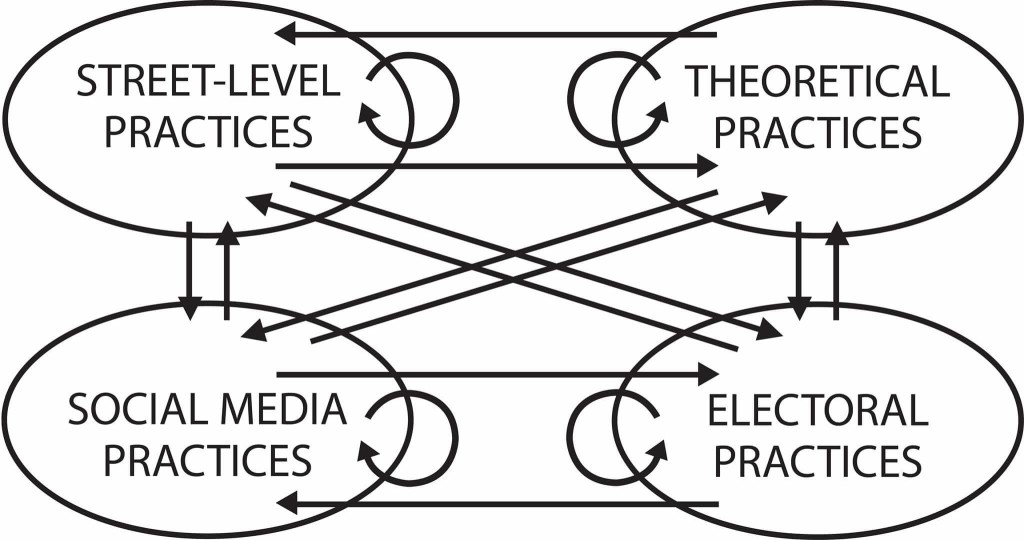
\includegraphics[width=.9\linewidth]{spheres-practices.png}
	\caption{Interacción entre prácticas electorales, teóricas, mediáticas y de calle.}
	\label{fig:interacciones}
	\todo[inline]{Valdria la pena rehacer un diagrama como este en español.}
\end{figure}

Una vez que logremos consolidar una infraestructura común y dinámicas para comunicarnos, es necesario que abramos canales de comunicación. Para lograrlo, podemos recurrir a estrategias muy antiguas, pero igualmente efectivas bajo una gran organización técnicamente capaz de hacer una democracia efectiva: Periodismo popular, repartido en lugares de resistencia a través de estructuras distribuidas por todo el país, donde los contenidos puedan enlazar realidades locales con la nacional. En realidad, la presencia de una organización política en el territorio no significa que haya buenas razones para ocuparlo, la razón por la que nos presentamos en la calle es quizá una de las cuestiones más importantes a resolver. Por ejemplo, adoptar una agenda municipalista sería un excelente horizonte para un movimiento que busca ocupar las instituciones del poder. Las propuestas de Murray Bookchin, ecologista estadounidense, pueden convivir con otros esfuerzos de organización comunitaria como los desarrollados por Saul Alisnky y Marshall Ganz. Quizá la razón más vital para salir a la calle sea la más poderosa. El carnaval, la festividad profana de lo público, la danza libre y el encuentro de los cuerpos, sería un gran pretexto. ¡Salgamos a la calle a divertirnos y hablar de lo político! También puede servir para redefinir nuestra concepción de un mercado libre y abierto.

Se pueden conciliar movimiento y elecciones a través de participación escalonada que se gestione a través de una plataforma web, así como plantear acciones importantes pero no urgentes para la organización y para desarrollar el movimiento. Esto para hacer una mancuerna operativa con las personas que consideran que conquistar espacios de poder es la tarea urgente, pero que estarían de acuerdo con abrir la organización para que están acciones importantes empiecen a ocurrir porque somos una wiki inteligente, que entiende el aspecto multidimensional de sus operaciones. Imaginamos una apertura escalonada de información, según lo que la gente quiera compartir y lo que la wiki haya ganado por su mérito de honorabilidad. \emph{Hay que entender que hoy es posible programar la gestión de responsabilidades orgánicamente.} Las alianzas deben permitirnos articular una red electoral, un plan de gobierno y un nuevo proyecto constitucional, desde una perspectiva abierta, transparente y \emph{FLOSS}. Consideremos que hay una asimetría en acceso a redes que hacen que gente menos experta o que ha pasado menos tiempo en la red tenga mayores dificultades para integrarse. Por esta razón no sabemos dar cauce a muchas ideas que son potencialmente grandes proyectos. Más allá de la preocupación porque un grupo de poder coopte la organización, hay que pensar que es necesario que el movimiento se fragmente y diferencie a partir de recursos comunes, bajo una visión modular y escalonada de los progresos de nuestra estructura política.

\begin{figure}[htbp]
	\centering
	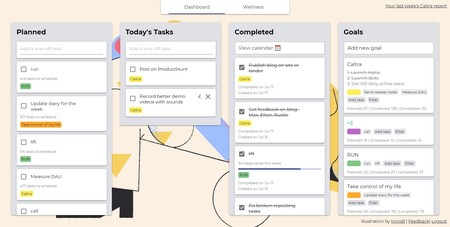
\includegraphics[width=.9\linewidth]{caltra.jpg}
	\caption{El sitio \url{www.caltra.co} te permite organizarte en listas y tableros.}
\end{figure}

El problema de la documentación de un movimiento político que busque la libertad real de todas las personas es una preocupación muy presente desde Podemos pero realmente constante a lo largo de la historia. El problema más importante hoy en día para los movimientos autogestionados se conoce como la \emph{tiranía de la no estructura.} Un problema difícil de enfrentar es que, en relación con el estado actual de las cosas, solo podemos ver lo que nos queda y muy pocas veces lo que nos ha sido arrebatado o todo lo posible, un horizonte imaginario de formas de organización, de diálogo, distintas. La cuestión de la inteligencia colectiva no puede quedarse como un instrumento más para agilizar la productividad. Mucha gente en Wikipolítica no se da cuenta lo útiles que resultan al Imperio con el burdo aceleracionismo de blancos por el que sienten tanta simpatía. Para hacer frente a estas cuestiones, necesitamos mecanismos para profesionalizar el activismo y la militancia, mecanismos de sistematización de experiencias. Partir de esto para diseñar un programa de crecimiento dirigido comprensivo y estratégico, una suerte de comunidad de inteligencia. Tenemos oportunidad de usar y desarrollar plataformas tecnológicas para gestionar procesos que ahora son inoperables bajo la tecnología que tenemos ahora. Para lanzar una campaña de crecimiento dirigida al territorio necesitamos despliegues de profesionales en Trabajo social en Comunicación. Es decir, necesitamos pensar estratégicamente. El problema es que entre muchas personas es moralmente incorrecto repetir

En Wikipolítica muchas veces nos preguntamos sobre las características de un posible espacio wiki oficial. Con el tiempo, estamos más convencidas que se trata de plantear qué significa un espacio wiki, preguntarnos cómo inspiramos a otras personas a crear espacios bajo una filosofía común. La ideología es la máscara a través de la cual vemos las cosas.

El diseño es parte de una propuesta de inteligencia que, a través de procesos de iteración y prueba, logra crear relaciones de experiencia entre las cosas y las personas. Creemos en el valor del Diseño como disciplina fundamental para la transmisión de un medio popular. Nuestro \emph{código} tiene que pensar en las instituciones a través del Diseño social. El resultado serán mecanismos que incentiven la participación más allá de la lógica utilitarista, fundamento de la magia negra. La única restricción serían las manifestaciones de totalitarismo, como la intolerancia, el autoritarismo o la intransigencia. Los discursos que atenten contra la determinación libre y voluntariosa de la persona deben ser contenidos y este es un límite al que no estamos dispuestas a renunciar.\footnote{El mejor remedio para los fascistas de sonrisa cínica y espíritu perverso es molerlos a palos. Pero nos conformamos con que sean expulsados.}

Por ejemplo, aprender a pensar en instancias para crear protocolos comunes de distintas luchas como las tecnologías de performance o la táctica del brigadeo. Operaciones orientadas a proyectos, donde las estructuras nazcan y mueran, sean ocupadas, como los hackerspaces. Metodologías de organización para y desarrollo para personas como SCRUM, design thinking, UX, grupos de agilismo, Workcafé. Otra tarea es consolidar un equipo de relatores que puedan sistematizar con rigurosidad los resultados de todas las discusiones, pues parece que la relatoría presupone más habilidades para la síntesis y la estructuración discursiva de lo que podría parecer.

La cuestión de una plataforma política puede funcionar muy bien como un proyecto modular de fuentes libres y abiertas basado en tecnologías que ya existen, como Decidim y las metodologías de gobernanza en círculos llamada Sociocracia. Con esta visión es muy factible desarrollar una estructura informática con directorios, sesiones de planificación y estrategias de mercado, asesoría para participar en convocatorias y solidaridad para que quienes quieran, se apoyen. Solo habría que considerar que el crecimiento esté dirigido estratégicamente hacia redes y personas clave en agendas específicas, además del mero crecimiento territorial. Necesitamos comprometernos con sentar un precedente operativo basado en nuestro potencial tecnológico. Si lo hacemos bien, la necesidad de apertura de otras asambleas políticas en el país se esparcirá como un meme (virus cultural), que permita que todas tengamos los saberes necesarios para organizarnos en torno a lo común.

En términos estratégicos, es mejor dar un golpe nacional de la nada, con precisión y organización, con artistas, académicos, opinión pública y otros sectores, que el desgaste que implica concentrarse en un solo proyecto de corto plazo, como una campaña política o una petición legislativa sin ninguna repercusión estructural. Mejor esperar unos años hasta que tengamos una organización poderosa. Abrir la organización con un movimiento nacional que siente las bases para un proyecto político fuerte y de larga duración.

Representación de convicciones políticas, agendas desde subjetividades reconocidas y desde los territorios. Burocracia media en sindicatos o partidos. Diferencia y relación entre sindicatos y partidos. Redes interuniversitarias. Necesitamos regulación de proyectos económicos a través de sus limitaciones. Es decir, si la industria editorial genera capital que se acumule en pocas manos (lo que significa menores ingresos tanto para escritorxs como para lectores), ser el espacio y respaldo de la innovación de nuevos modos de financiamiento, quizá haciendo hackatones o dando prioridad al tema en las agendas de un período y una región en particular. Hackatones sociales o alguna iniciativa donde podamos ser facilitadoras de distintos fondos públicos locales. En el terreno económico podemos jugar el papel de gestoras para cooperativas de consumo que compartan una identidad y principios wiki que permitan que muchas familias puedan empezar a adquirir sus bienes en redes sororas.

\section{¿Cómo entender los problemas de nuestro país?}
\label{sec:problemaspais}

El Estado en México es un orden social de acceso limitado, hay que
pensar en systems thinking para crear un frame que comprenda necesidades
para ajustar la plataforma política al contexto de institucionalidad y
reglas del juego propias de cada arreglo. Habría que partir de una
visión combinada de psicoanálisis, diseño y economía de la conducta. Hay
que hacer una lista de problemas principales a resolver, por ejemplo:

\subsection{Problemas de diseño de sistemas:}
\label{sec:probsis}

\begin{itemize}
	\item Interfaces y experiencia de usuario comunitarias y accesibles

	\item Teoría del empujón para incentivos económicos a cooperativas y apropiaciones comunitarias del espacio público
\end{itemize}

\subsection{Problemas de acción colectiva}
\label{sub:probaccion}

\subsubsection{Económicos}
\label{subs:economicos}

\begin{description}
	\item[Asimetrías de información:] cómo hacemos que la gente tenga los mismos insumos para tomar las decisiones más benéficas para las comunidades en un mercado complejo de transacciones en tiempo real

	\item[Problema del agente-principal:] abolir las altas tasas cobradas por coyotes que dan sentido a la figura del Estado como recaudador central que redistribuye el ingreso

	\item[Tiranía de la no estructura:] sistemas de toma de decisiones para la participación escalonada y remunerada de diferentes agentes con un objetivo común de solidaridad económica

	\item[Comunes:] formalización en protocolos y procesos de una cultura de los bienes y servicios comunes que se gestionan, se actualizan y se mantienen a través de contribuciones pre-establecidas en contratos inteligentes
\end{description}

\subsubsection{Psíquicos}
\label{subs:psiquicos}

\begin{description}
	\item[\emph{Schadenfreude}:] cómo crear grupos de personas con adicciones, resentimientos o comportamientos tóxicos que sienten placer por el sufrimiento del prójimo, y comenzar procesos de sanación colectiva descentralizados, como Alcohólicos Anónimos.

	\item[Narcisismo de las pequeñas diferencias:] Construcción de una cultura política que procure las alianzas y permita canalizar los disensos. Un ejemplo muy claro para la construcción de organizaciones que hagan frente a este tipo de cuestiones es la Sociocracia.
\end{description}

\begin{figure}[htbp]
	\centering
	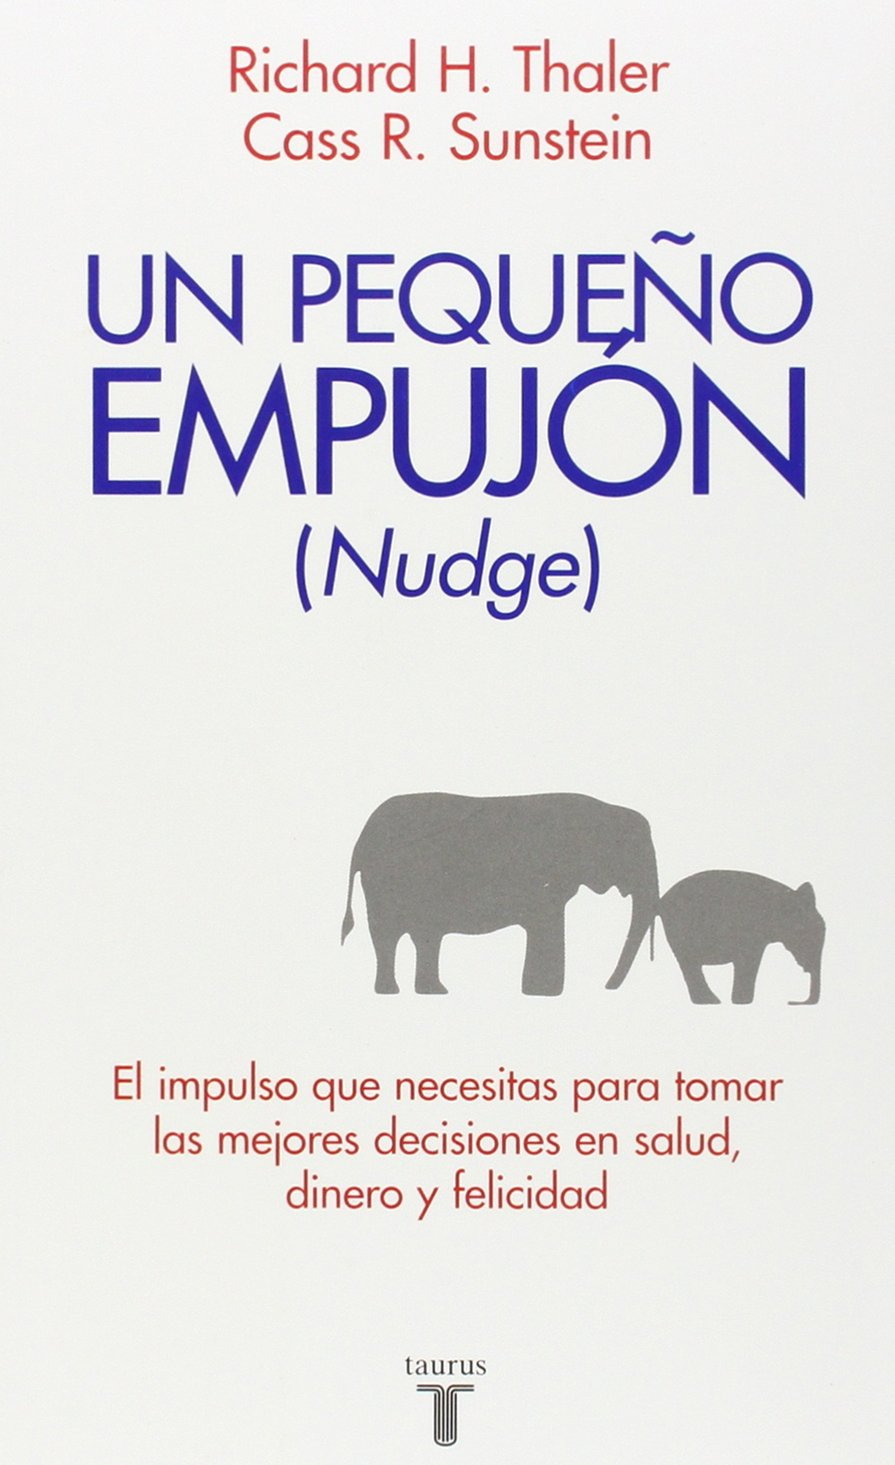
\includegraphics[width=.9\linewidth]{nudge.jpg}
	\caption[\emph{Nudge}]{El libro \emph{Nudge} es una gran referencia para entender el poder del diseño y la economía del comportamiento en la solución de problemas públicos.}
	\label{fig:nudge}
\end{figure}

\section{Consideraciones sobre la organización}
\label{sec:considerorga}

Las herramientas ya existen, es poco trabajo en interconectarlo (compatibilidad de tecnología), hay que enfocarnos en la adopción a través de talleres y eventos de accesibilidad, de editorializar una base de datos opinionated suite de trabajo militante), de garantizar protocolos de seguridad: decentralizacion, permisos (gestion de identidad) (Pursuance, sneakernet y otras tecnologías). Tenemos que desarrollarlo poco a poco a través de una arquitectura modular y distribuida, que permita ensamblar diferentes tecnologías según las necesidades de la persona usuaria.

El problema principal para un movimiento horizontal es el problema de la \emph{no-estructura}.\revquotes{} Dentro de las estrategias, podemos proponer visiones para que los emprendedores entiendan como disruptivo lo que es estructural. Se trata de reapropiarse del concepto de "gobernanza"dinámica y participativa, pensar que sea una gobernanza basada en \hlfix{outputs}{En cursivas.} o resultados sin que se vuelva una cosa individualista de \hlfix{tracking}{Ibid.} de \hlfix{performance}{Ibidem.} individual. El objetivo es crear una estructura de los comunes (Elinor Ostrom), además de fortalecer sindicatos, acelerar cooperativas y democratizar decisiones corporativas, facilitar \hlfix{self-management}{Ibid.} y \hlfix{self-organization}{Ibidem.} en un movimiento \hlfix{antileadership}{Ibid.}.

Para lograrlo hay que retomar la paradoja de la sistematización de actividades ¿creamos y documentamos procesos o patrones? ¿Realmente vale la pena un modelo de gobernanza como sociocracia?

Recursos interesantes para este apartado:

Github: The GitHub Debacle and Why Holacracy is Bullshit
(counter-response)
\url{http://cbracy.tumblr.com/post/79876957198/the-github-debacle-and-why-holacracy-is-bullshit}
\chapter{¡Accionemos!}
\label{cha:accionemos}

¿Qué podemos hacer? Nuestra posición es una práctica pragmática y eficaz desde el xenofeminismo como filosofía de inspiración de La Partida. Más allá de la coherencia moral, nos interesa agruparnos con formas de vida que nos hagan potentes, es decir, en las formas de vida que procuran el cuidado, el bien común. Por ahora, con nuestra agencia limitada por la poca credibilidad de la juventud, nos toca infiltrarnos e incidir en diferentes medios, en partidos políticos, organizaciones internacionales, medios de comunicación masiva y segmentada, entre otras estructuras.

\begin{figure}[htbp]
	\centering
	
\includegraphics[width=0.7\linewidth]{leo-silvestri.jpg}
	\caption[Leonor Silvestri]{Leonor Silvestri, feminista argentina y activista de los afectos alegres con excelentes reflexiones en YouTube.}
	\label{fig:silvestri}
\end{figure}

\section{Algunas posibles acciones estratégicas}
\label{sec:posiblesacciones}

Un Centro de Estudios que brinde a las personas que estudian ahí capacidades de formación en medio de la complejidad y que formen generaciones dispuestas a accionar desde una perspectiva transdisciplinaria y colaborativa, lejos de los dogmas y formalismos de la academia. Como el proyecto de Nick Srnicek con Hellen Hester, autonomy.work. Dentro de los proyectos claves vemos:

Un \emph{think tank} para generar líderes con conciencia crítica, de estrategia y táctica política, además de informes de política económica de desarrollo local y estrategias para hubs y hackatones, además de programas de litigio estratégico rumbo a la creación de un programa de políticas publicas poscapitalista. Necesitamos crear lazos con los entornos tecnológicos progresistas y radicales para poder crear productos accesibles en los mercados que puedan generar bienestar para muchas personas, por ejemplo, a través de franquicias cooperativas.

\begin{figure}[htbp]
	\centering
	
\includegraphics[width=0.6\linewidth]{autonomyWork.png}
	\caption{Logo del \emph{think tank} comenzado por Hellen Hester y Nick Srnicek, \texttt{autonomy.work}.}
	\label{fig:autonomywork}
\end{figure}

Ademas, necesitamos crear una plataforma de organización política en línea de arquitectura modular que sea accesible y fácil de implementar. Un excelente punto de partida es el proyecto Decidim desarrollado en el MediaLab en España. Nos imaginamos las bases de una interfaz para discusión y gestión democrática de grupos, además de una wiki que funcione como un repositorio copyfair editorializable. Ademas, con tecnologías de georreferenciación.

En términos económicos, hay que crear un ecosistema que facilite la proliferación y producción de redes solidarias. Más allá del movimiento sindicalista, la cooperativa es una unidad económica que realmente garantiza la igualdad democrática desde el trabajo. Quizá la forma más sencilla de hacerlo sería a través de una franquicia cooperativista cuyo soporte sea una wiki con manuales y procesos accesibles en términos de diseño, que crezca bajo una etiqueta (\emph{label}) que represente los valores de esa marca cooperativa.\footnote{Un ejemplo del crecimiento rizomático de una organización es la nevería mexicana La Michoacana.}

Finalmente, es necesario desarrollar un proyecto cultural transmedia que funcione a través de esta lógica y que permita el desarrollo de una cultura popular independiente del mercado \emph{mainstream}. Algo de inspiración para una aventura de esta naturaleza han sido los \emph{Street papers} y proyectos como la Red de Producción y Distribución Vicente Guerrero en México, el manifiesto del Dogma 95 y el formato de producción de bajo costo desarrollado por Robert Rodriguez en su famoso libro \emph{Rebel without a Crew}. En resumen, una cultura de producción \emph{guerrilla cinema}. Las películas \emph{Tangerine} en Estados Unidos y \emph{Oso Polar} en México son una muestra de las posibilidades técnicas de los medios contemporáneos. Sin embargo, el horizonte de un esquema de producción audiovisual militante es ContraPoints, un vlog en YouTube estelarizado por Natalie Wynn.

\begin{figure}[htbp]
	\centering
	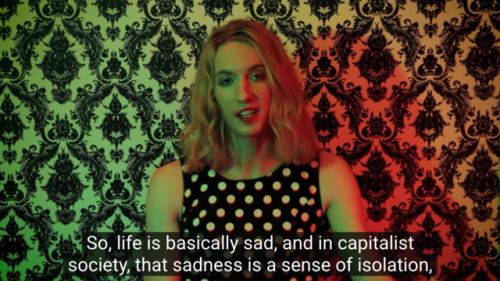
\includegraphics[width=.9\linewidth]{contrapoints.png}
	\caption[Natalie Wynn.]{Natalie Wynn, creadora de ContraPoints.}
	\label{fig:Wynn}
\end{figure}


\section{Organízate e independízate del Capital}
\label{sec:independizate}

Finalmente, lo más importante es encontrar la forma de compartir recursos que nos permitan crear redes de solidaridad en la producción de insumos clave para cubrir necesidades básicas de grupos y comunidades. En un sentido meramente estratégico, la pirámide de Maslow nos da pistas de las industrias que habría que comenzar a cooperativizar para crear multitudes que se emancipen de los flujos farmacopornográficos, chatarrofágicos y financieros que produce el capitalismo.

\begin{figure}[htbp]
	\centering
	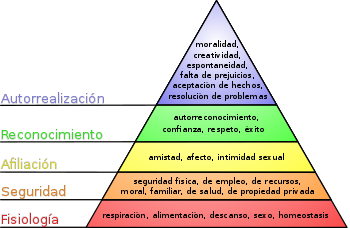
\includegraphics[width=.9\linewidth]{maslow.png}
	\caption{Pirámide de Maslow sobre necesidades.}
	\label{fig:maslow}
\end{figure}

Económicamente, problemas como el hambre o la vivienda pueden resolverse con técnicas avanzadas de planificación y coordinación que no podían realizarse en el socialismo de hace casi un siglo por la sencilla razón de que no contaban con las herramientas computacionales necesarias para poder pensar con seriedad en una economía planificada que publique precios y soluciones conflictos de asimetrías de información en el mercado.

Hoy tenemos la capacidad de no solo permitir la proliferación organizada en plataformas comunes de productoras descentralizadas que surtan en función de necesidades y no de plusvalía financiarizable, también podemos implementar sistemas de votación para que estas organizaciones no sean, como lo fueron durante la revolución mexicana, la base de un corporativismo de corte charro. Podemos crear plataformas de economía solidaria capaces de gestionarse autónomamente a través de recursos iterativos de código FLOS. En ese sentido, una etiqueta de franquicia cooperativa sería una buena forma de crear documentación y procesos comunes en un proyecto de riesgo compartido con un contrato claro e incluso inteligente y encriptado.

\appendix
\backmatter

\chapter{Anexos}
\label{cha:anexos}

\section{Territorios de prácticas participativas}
\label{sec:territorios}

Actualmente estoy dividiendo la información en un gran conjunto de Diagramas de Venn (en realidad más bien Esferas de Venn):\footnote{Traducido con \url{www.deepl.com/translator} desde \url{www.github.com/ParticipatoryOrgs/Participatory-Organizations-Overview-and-Taxonomy}}

La esfera más grande es la de los Ecosistemas Participativos, que tienen una serie de prácticas para apoyar los sistemas regenerativos de un bien común, así como una política cultural para aumentar la participación a todos los niveles, y para incentivar contra la tragedia de los bienes comunes y la desigualdad en la equidad.

Dentro de esa esfera se encuentran dos esferas de Venn, las Corporaciones Participativas y las Organizaciones Participativas. Tienen mucho en común, pero las Corporaciones Participativas tienen más que ver con el mantenimiento y crecimiento del capital financiero, mientras que las Organizaciones Participativas están más enfocadas en el mantenimiento y crecimiento de las comunidades.

Dentro de la intersección de las esferas de las Corporaciones y Organizaciones Participativas hay un número de burbujas más pequeñas. Hay una gobernanza participativa, operaciones participativas y una visión y cultura participativas.

La gobernanza participativa aumenta el compromiso de las partes interesadas al hacerlas participar en la elaboración de políticas. Existe una gran variedad de estos procesos. Lo que se conoce como \emph{Toma de Decisiones por Consenso} es una esfera que está más cerca del lado de las Organizaciones Participativas, pero también cerca del lado de la Visión. Hubo bastante innovación en estos procesos en el movimiento \emph{New Paradyne Management} que terminó a mediados de los 90 debido al boom de las \emph{punto com} que no requirió una gran participación o incluso una gran gestión.

Operaciones Participativas se centra más en tener más ojos en las tácticas y la logística. Los procesos Lean y Agile encajan aquí, Intrapreneuring puede así como una serie de otros procesos de gestión de proyectos.

La Gobernabilidad Dinámica es una esfera de Venn que se encuentra mayormente dentro de la Gobernabilidad Participativa, pero más cerca del lado de las Operaciones Participativas que del lado de la visión. Dentro de eso está la Sociocracia que se inclina fuertemente hacia las Organizaciones Participativas en la preservación del capital comunitario y social y también cerca de la Visión y Cultura Participativa. La Holacracia es también una forma de Gobierno Dinámico, pero se inclina hacia el lado corporativo, pero también trata de funcionar mucho más en el espacio de Operaciones Participativas. La Holacracia apoya más la esfera de la Política que las Operaciones. La sociocracia también apoya más a la esfera de la política, pero en gran medida da flexibilidad a la esfera operativa.

Las prácticas participativas pueden dividirse en 3 grandes áreas: Sistemas participativos, participatory equity y gobernanza participativa.

Algunos principios:\todo{¿y por qué en inglés?}

\begin{itemize}
\item \emph{Act}: You Already Have Permission
\item \emph{Flow}: Every Idea Is Playdough
\item \emph{Open}: Everything Is Transparent
\item \emph{Accept}: It Isn't Easy Being Green
\item \emph{Share}: Communication Is Oxygen
\end{itemize}

\begin{figure}[htbp]
	\centering
	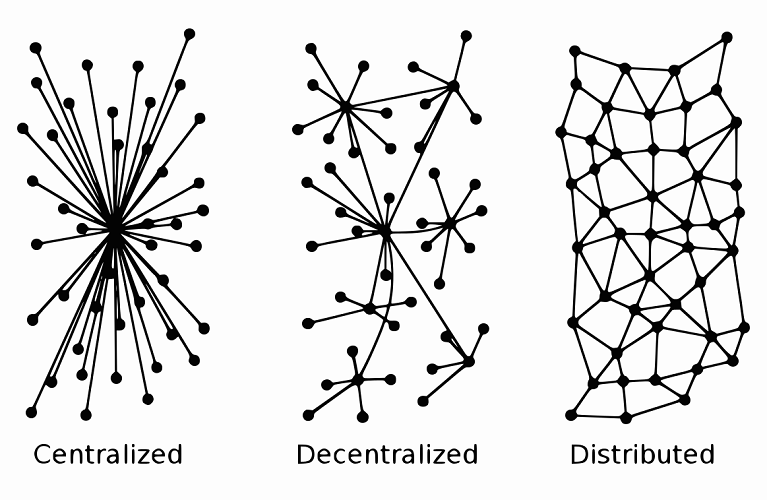
\includegraphics[width=.9\linewidth]{decentralized.png}
	\caption{Centralizado, descentralizado, distribuido.}
	\label{fig:descentralizado}
\end{figure}

\section{Tiranía de la falta de estructuras}
\label{sec:tirania}

Es importante enfatizar el patrón negativo discutido en el famoso ensayo de Jo Freeman de 1970 \emph{The Tyranny of Structureless}. Usando las lecciones del movimiento feminista de los años 60, evitar la estructura puede en realidad reforzar las estructuras, y a menudo de manera no beneficiosa, enmascarando los abusos de poder:

\begin{quotation}
	Contrariamente a lo que nos gustaría creer, no existe tal cosa como un grupo sin estructura. Cualquier grupo de personas de cualquier naturaleza que se reúna por cualquier período de tiempo y con cualquier propósito se estructurará inevitablemente de alguna manera. La estructura puede ser flexible; puede variar con el tiempo; puede distribuir las tareas, el poder y los recursos entre los miembros del grupo de manera uniforme o desigual. Pero se formará independientemente de las habilidades, personalidades o intenciones de las personas involucradas. El hecho mismo de que somos individuos, con diferentes talentos, predisposiciones y antecedentes, hace que esto sea inevitable. Sólo si nos negamos a relacionarnos o a interactuar sobre cualquier base, podremos aproximarnos a la falta de estructura - y esa no es la naturaleza de un grupo humano.

	Esto significa que luchar por un grupo sin estructura es tan útil y engañoso como apuntar a una noticia \emph{objetiva}, a una ciencia social \emph{sin valor} o a una economía \emph{libre}. Un grupo de laissez faire es tan realista como una sociedad de \emph{laissez faire}; la idea se convierte en una cortina de humo para que los fuertes o los afortunados establezcan una hegemonía incuestionable sobre otros. Esta hegemonía puede establecerse tan fácilmente porque la idea de falta de estructura no impide la formación de estructuras informales, sólo formales. De manera similar, la filosofía del \emph{laissez faire} no impidió que los económicamente poderosos establecieran el control sobre los salarios, los precios y la distribución de los bienes; sólo impidió que el gobierno lo hiciera. Por lo tanto, la falta de estructura se convierte en una forma de enmascarar el poder, y dentro del movimiento de las mujeres es por lo general más fuertemente defendido por aquellos que son los más poderosos (sean o no conscientes de su poder). Mientras la estructura del grupo sea informal, las reglas de cómo se toman las decisiones son conocidas sólo por unos pocos y la conciencia del poder se limita a aquellos que conocen las reglas. Aquellos que no conocen las reglas y no son elegidos para la iniciación deben permanecer confundidos, o sufrir de delirios paranoicos de que algo está sucediendo de lo que no son del todo conscientes.
\end{quotation}

También:

\begin{itemize}
\item \url{http://www.wired.com/2014/03/tyranny-flatness/}
\item \url{https://en.wikipedia.org/wiki/Flat\_organization\#Criticisms}
\item \url{https://theanarchistlibrary.org/library/cathy-levine-the-tyranny-of-tyranny}
\end{itemize}

\section{Bienes comunes}
\label{sec:org695eb10}

Las organizaciones participativas suelen tener que gestionar recursos en común al interior de la organización en su conjunto (activos, presupuestos, tiempo, etc.), o están participando en bienes públicos compartidos pero limitados que, junto con otras organizaciones, pueden ser tangibles (aire, recursos, etc.) o intangibles (conocimiento, código abierto, etc.).

En 2009, Elinor Ostrom recibió el Premio Nobel de Economía por su análisis de la gobernanza económica, especialmente de los bienes comunes. En ese sentido, enumeró ocho principios para una gestión eficaz contra la tragedia de los bienes comunes. Estos son muy útiles para las organizaciones participativas:

\begin{enumerate}
	\item[1A.] Definir el uso autorizado

	\item[1B.] Definir los límites de los bienes comunes

	\item[2A.] Hacer que los costes sean proporcionales

	\item[2B.] Pagar todos los gastos

	\item[3A.] Decidir inclusivamente

	\item[3B.] Adaptarse localmente

	\item[4A.] Compartir conocimientos

	\item[4B.] Monitoreo efectivo

	\item[5 .] Responsabilizar (\emph{hold accountable})

	\item[6 .] Resolver rápidamente los conflictos

	\item[7 .] Gobernar localmente

	\item[8 .] Conectar y coordinar con sistemas relacionados
\end{enumerate}

\section{Referencias del apartado}
\label{sec:ref07}

\begin{itemize}
	\item How Commons Can Flourish: \url{https://commons.blog/2012/08/18/how-commons-can-flourish/}
	\item The Antifragile: Things That Gain from Disorder: \url{https://cpor.org/af/Taleb\_Antifragile.pdf}
	\item Herramientas del partido pirata argentino: \url{https://utopia.partidopirata.com.ar/democracia\_directa.html}
	\item Algoritmos para predecir cooperación social: \url{http://news.harvard.edu/gazette/story/2017/03/harvard-scientists-help-develop-algorithm-that-predicts-social-cooperation/}
	\item Movimiento OPEN: \url{http://open.co/}
	\item Agentes de innovación en México - CIDE: \url{https://es.slideshare.net/mobile/DapCide/advancing-innovation-mexicos-innovation-agents-eng} 
	\item Ciencia de redes, por Laszlo Barabási: \url{http://barabasi.com/networksciencebook/}
	\item Marcos para diseño organizacional: \url{http://isites.harvard.edu/fs/docs/icb.topic608877.files/Class\%20Nine\%20Reading/CLC\_Frameworks\_for\_Organizational\_Design.pdf}
	\item De capos y rodeos, ¿por qué nada funciona?: \url{https://www.northatlanticbooks.com/blog/of-warlords-and-rodeos-why-nothing-works/}
	\item Problem Driven Iterative Adaptation (vs other mainstream approaches for public policy): \url{https://www.hks.harvard.edu/index.php/centers/cid/programs/building\_state\_capability/what-is-pdia}
	\item \url{https://framasoft.org}
	\item \url{http://unenumerated.blogspot.com/2017/02/money-blockchains-and-social-scalability.html}
	\item \url{http://unenumerated.blogspot.com/2006/11/wet-code-and-dry.html}
\end{itemize}
\cleardoublepage

\layout 
\end{document}